%-----------------------------------------------------------------------------
%
%               Template for sigplanconf LaTeX Class
%
% Name:         sigplanconf-template.tex
%
% Purpose:      A template for sigplanconf.cls, which is a LaTeX 2e class
%               file for SIGPLAN conference proceedings.
%
% Author:       Paul C. Anagnostopoulos
%               Windfall Software
%               978 371-2316
%               paul@windfall.com
%
% Created:      15 February 2005
%
%-----------------------------------------------------------------------------


\documentclass[]{sigplanconf}

% The following \documentclass options may be useful:
%
% 10pt          To set in 10-point type instead of 9-point.
% 11pt          To set in 11-point type instead of 9-point.
% authoryear    To obtain author/year citation style instead of numeric.

\usepackage{amsmath}
\usepackage{graphicx}
\usepackage{url}
\usepackage{amssymb}
\usepackage{subfigure}
\usepackage{algorithm} 
\usepackage{algpseudocode}
%\usepackage{times}

% make an environment for subfigures with verbatim
\newbox\subfigbox	% Create a box to hold the subfigure. 
\makeatletter
  \newenvironment{subfloat}% % Create the new environment. 
    {\def\caption##1{\gdef\subcapsave{\relax##1}}%
    \let\subcapsave=\@empty % Save the subcaption text.  
    \let\sf@oldlabel=\label 
    \def\label##1{\xdef\sublabsave{\noexpand\label{##1}}}%
    \let\sublabsave\relax  %
    \setbox\subfigbox\hbox 
        \bgroup}% 
     {\egroup   %
    \let\label=\sf@oldlabel
    \subfigure[\subcapsave]{\box\subfigbox}}% 
\makeatother

\newcommand{\eightpoint}{\fontsize{8pt}{10pt}\selectfont}
\newcommand{\ninepoint}{\fontsize{9pt}{11pt}\selectfont}

\advance \baselineskip by 0.4pt

% do not indent paragraphs of enumerated lists (my lists go on for pages...)
% numbers flush left to paragraph text: \leftmargin=17pt
\newcommand{\mybegin}{\begin{list}{\labelenumi}{\leftmargin=\parindent}\usecounter{enumi}}
%\newcommand{\myitem}[1]{\item {\textit{\textbf{#1}}}}
\newcommand{\myitem}[1]{\item {\bf #1}}
\newcommand{\myend}{\end{list}}
\newcommand{\mt}[1]{\mbox{\it #1}}
\newcommand{\todo}[1]{\framebox {\bf #1}}



\begin{document}

%\conferenceinfo{PLDI  2011}{June 2011, San Jose, CA.} 
%\copyrightyear{2010} 
%\copyrightdata{[to be supplied]} 

%\titlebanner{banner above paper title}        % These are ignored unless
%\preprintfooter{short description of paper}   % 'preprint' option specified.

\title{Sliding Window Computations in Stream Programs}
%\subtitle{Subtitle Text, if any}

\authorinfo{}
           {}
            {}
% \authorinfo{Name2\and Name3}
%            {Affiliation2/3}
%            {Email2/3}

\maketitle
\begin{abstract}
Due to the high data rates involved in audio, video, and signal
processing applications, it is imperative to compress the data to
decrease the amount of storage used.  Unfortunately, this implies that
any program operating on the data needs to be wrapped by a
decompression and re-compression stage.  Re-compression can incur
significant computational overhead, while decompression swamps the
application with the original volume of data.

In this paper, we present a program transformation that greatly
accelerates the processing of compressible data.  Given a program that
operates on uncompressed data, we output an equivalent program that
operates directly on the compressed format.  Our transformation
applies to stream programs, a restricted but useful class of
applications with regular communication and computation patterns.  Our
formulation is based on LZ77, a lossless compression algorithm
utilized by ZIP, and immediately applies to simpler formats such as
Apple Animation, Microsoft RLE, and Targa.

We implemented a simple subset of our techniques in the StreamIt
compiler, which emits executable plugins for two popular video editing
tools: MEncoder and Blender.  For common operations such as color
adjustment and video compositing, computing directly on compressed
data offers a speedup roughly proportional to the overall compression
ratio.  For our benchmark suite of 12 videos in Apple Animation
format, speedups range from 1.1x to 471x, with a median of 15x.

\end{abstract}

%\category{CR-number}{subcategory}{third-level}

%\terms
%term1, term2

%\keywords
%keyword1, keyword2

\section{Introduction}


Stream computing represents an increasingly important class of
applications. In streaming codes, there is an abundance of parallelism that
is easier to extract compared to traditional desktop workloads (e.g.,
pointer-based computing). As a result, the extraction of parallelism
in streaming codes does not require heroic efforts, and thus,
processors can deliver higher performance with significantly lower
power costs. This is especially important since
leading microprocessor companies have realized that modern general
purpose architectures are near their  performance limits for  the
amount of power they consume. Thus, the future will place a greater
emphasis on exploiting the properties of streaming workloads in
conventional von~Neumann architectures.

Streaming is a model of computation that uses sequences of data
and computation kernels to expose concurrency and locality for
efficiency~\cite{wss}. In general purpose processors, improving locality 
translates to an effective management of the memory hierarchy at all
levels, including the register file. In this paper, we present a
methodology for compiling streaming codes to general purpose,
cache-based architectures. We first introduce a simple model for
reasoning effectively about the caching behavior of streaming
workloads. This model serves as a foundation for several {\it cache-aware
optimizations} that are geared toward the concomitant increase of instruction
and data {\it temporal locality}. These
optimization lead to significantly better utilization of the memory
system, and as such, they deliver performance gains ranging from 11
to 99\% for our streaming benchmark suite.

The context for our work is StreamIt, an architecture-independent
language that is engineered for streaming
applications~\cite{streamitcc}. It adopts the 
Cyclo-Static Dataflow~\cite{BELP96} model of computation which is a
generalization of Synchronous Dataflow~\cite{LM87-i} (SDF).  
SDF is a popular  model that  is well suited for
streaming codes. In SDF, computation is represented as a graph
consisting of {\it  actors} connected by communication channels; the
actors consume  and produce a constant number  of items from their
input and output  channels every time they execute. SDF is appealing
because it is amenable to static scheduling and optimization. 

From a general purpose architecture's point of view, actors represent
computation kernels, and the communication between actors represents
data buffers that must be streamed to and from the processor. Thus
the size of an actor and the
order of actor executions are critical properties that
impact the performance of the instruction cache. For example, the
compiler must make sure the actor's code size is not
greater than the instruction cache. Furthermore, we must {\it scale}
the execution of the actor so that it runs several times before we move
on to some other actor in the stream 
graph. This serves to $(i)$ amortize the cost of fetching the actor's
instructions into the cache from memory (an expensive operation), $(ii)$
improve the instruction temporal locality, and $(iii)$ improve overall
performance. However, as our cache model will show, we 
cannot arbitrarily scale the execution frequency of an actor. This
is because actors produce data that must be buffered, and therefore,
we must also consider the amount of data an actor produces and
consumes if we are to adequately manage the data cache. This paper is unique
in that it is the first to present a unified optimization methodology
that simultaneously considers instruction and data locality for
mapping streaming computation to cache-based architectures.

In terms of improving the data cache behavior, the compiler schedules
actor firing such that the producer-consumer locality is
preserved. Furthermore,  the compiler may {\it fuse}
together two or more actors to form a coarser grained kernel.
The fusion allows for better register allocation as we can
destroy the arrays used to buffer data between the actors and replace
the corresponding array references with scalars.  It also allows for
various competing implementations for managing the buffers between the
fused actors.  This paper evaluates several implementation
alternatives (for buffer management) and evaluates their performance.

The methodology for fusing actors leverages a distinguishing StreamIt
characteristic, namely, the hierarchical organization of
the stream graph. Furthermore, the algorithm for fusing actors applies
for the various topologies allowed by StreamIt.
It also considers another distinguishing characteristics of StreamIt,
namely the {\tt peek} operation whereby an actor may inspect data
items in its input buffer without consuming them until some future
execution. While peeking is a powerful language feature, it does pose
some challenges to the compiler and the cache optimizations. Peeking
also impacts the choice for the best buffer management strategy, as our
study will show.

%% the comment about p3 and itanium not being embedded architectures
%% is out of the blue! need a better transition.
Cache-aware fusion alone delivers significant performance gains, although our
evaluation shows that fusion with scaling leads to the best
performance on a general purpose, cache-based architecture. For our
experiments, we use two different processors: a superscalar out-of-order
processor, and an in-order VLIW processor. The former is a Pentium~3
whereas the latter is an Itanium~2. While these architectures are not
particularly suited for an embedded system, they do exhibit some
properties that are worthy of investigation. Furthermore, that we can
demonstrate measurable performance gains on real systems is far more
convincing than using a simulation-based environment. We chose the
Pentium~3 processor because it has very few registers in its
instruction set architecture. The Itanium by contrast has a much 
larger and richer repertoire of registers. The two architectures serve
to validate our cache-aware optimizations, in that we expect an
architecture with more register to benefit more from optimization such
as scalar replacement. On average, fusion leads to a 47\% improvement
on the Pentium~3, and 50\% on the Itanium~2.

The two architectures also differ in terms of their memory system
organization. The Itanium is an in-order VLIW processor and does not
tolerate a memory stall as well as its out-of-order
counterpart. Therefore we expect different gains from the scaling
optimization which amortize the long access latencies for instruction
and data caches. On average, scaling leads to a 21\% improvement on
the Itanium~2, and 17\% on the Pentium~3.

While both scaling and fusion lead to modest performance gains, we
must combine the two to deliver the best possible performance. When we
do so, we can further improve the performance of our benchmarks by
53\% on average for the Pentium~3, and 55\% for the Itanium~2.

\subsection{Summary of Contributions}

This paper makes the following contributions:
\begin{itemize}

\item A cache model for stream computing that provides a quantitative
estimate of the caching performance for any sequence of actor
executions.

\item A cache-aware scheduling heuristic that judiciously increases
the multiplicity of actors, improving instruction and data locality
while not exceeding the data cache.

\item A cache-aware partitioning policy that judiciously fuses
adjacent actors into a single component, enabling local optimizations
while not exceeding the instruction cache.

\item An optimized buffer management policy, termed ``copy-shift with
execution scaling'', which out-performs a traditional rotating buffer
in a detailed micro-benchmark analysis.

\item A fully automatic implementation of the above techniques in the
StreamIt compiler.

\item An experimental evaluation across 11 streaming benchmarks,
demonstrating performance improvements of up to 99\%.
\end{itemize}

\subsection{Paper Roadmap}

The remainder of the paper is organized as follows. Section~\ref{sec:streamit}
describes StreamIt and introduces our motivating example.
Section~\ref{sec:cache-model} introduces our cache model for 
reasoning about the performance of a streaming
computation. Section~\ref{sec:cache-opt} describes our cache-aware
optimizations, and Section~\ref{sec:buffer} describes the 
optimization enabled by fusion. Section~\ref{sec:evaluation} describes
our evaluation methodology and present our experimental
analysis. Sections~\ref{sec:related-work}~and~\ref{sec:conclusion}
discuss related work and concludes the paper.

%% \begin{figure}
%% \centering
%% \psfig{figure=tapes.eps,width=2.5in}
%% \caption{A filter's input and output tapes during an execution step.
%% With each step, the filter pushes two items, pops two items, and peeks
%% at three additional items.  The initial state of the input tape is
%% shown at left.  The center shows the filter with both input and output
%% tapes during the invocation of {\tt work}.  The final state of the
%% output tape is shown at right.}
%% \label{fig:tapes}
%% \end{figure}

\begin{figure}
\centering
\psfig{figure=pipeline.eps,width=1.76in}

(a) A Pipeline. \\
\vspace{8pt}
\psfig{figure=splitjoin.eps,width=3.0in}

(b) A SplitJoin. \\
\vspace{8pt}
\psfig{figure=feedback.eps,width=2.33in}

(c) A FeedbackLoop. \\
\caption{StreamIt structures with labeling.}
\vspace{-12pt}
\label{fig:tapelabels}
\end{figure}

\section{Streaming Model of Computation}

In this section, we develop an abstract model of streaming computation
to serve as a basis for reasoning about program transformations and
compilation techniques within the streaming domain.  A stream graph
differs from a traditional, sequential program in that all of the
filters of the graph are implicitly running in parallel, with the
execution order constrained only by the availability of data on
channels between the filters.  Further, filters communicate only with
their immediate neighbors, thereby removing any notion of global time
or non-local dependences of one filter on another.  [add idea that it
is the specification of the atomic work function that really prevents
global time] These properties merit the development of a new model of
computation, in which the notions of timing, scheduling, and
dependence analysis are in terms that are relative to a given filter
in the graph, instead of being global characteristics of a program.

In Section \ref{sec:minfunc}, we develop a transfer function that
provides the basis for distributed time in a stream graph... [build
operational semantics to give a precise meaning to messaging, and
denotational semantics to validate program transformations].

\subsection{Notation}

We use the following notation:

\begin{itemize}

\item A {\it tape} is an infinite history of the values that have been
  pushed onto a channel between two filters. We use $I_S$ and $O_S$ to
  denote the input and output tapes of stream $S$, respectively, with
  numbering used to distinguish between multiple input or output tapes
  (see Figure \ref{fig:tapelabels}).  Finally, $n(T)$ represents the
  number of items on tape $T$ at a given point of execution.  [should
  we define $p(T)$ here or wait until we use it?  long time def-use!]

\item We say that a filter $A$ is {\it upstream} of filter $B$ (or,
  equivalently, $B$ is {\it downstream} $A$) if there is a directed
  path in the stream graph from $O_A$ to $I_B$.  We use this
  terminology for tapes as well as filters.

\item The number of items that are pushed, popped, and peeked by
  filter $A$ during a single execution of its work function are
  denoted by $push_A$, $pop_A$, and $peek_A$, respectively.  Note that
  $peek_A$ includes the items that are popped, such that $pop_A \le
  peek_A$.

\end{itemize}

\subsection{Relative Time}
\label{sec:minfunc}

As outlined above, there is no concept of global time in a stream
graph since each filter is completely independent and can only
communicate with its neighbors through input and output channels.
Thus, if two filters need to synchronize an event, the synchronization
must be in terms of the data items that are passed over a channel.

In this context, we define a $min$ function between tapes in the
stream graph that allows disconnected filters to have a common notion
of time.  The function is defined in terms of data dependence:
\begin{definition}
$\mi{a}{b}(x)$ is the minimum number of items that must appear on tape
$a$ given that there are $x$ items on tape $b$.
\end{definition}
We now turn to deriving $\mi{a}{b}$ for all pairs of tapes $a$ and $b$
in a filter graph where $a$ is upstream of $b$.

\subsubsection{Filters}

Let us derive $\mi{I_A}{O_A}(x)$, which represents the time shift
across a single filter $A$.  Since the filter produces $push_A$ items
on every invocation, it must be invoked
$\left\lceil\frac{x}{push_A}\right\rceil$ to produce the $x$'th item.
On each invocation, it consumes $pop_A$ items, and peeks at an
additional $peek_A-pop_A$ items.  Thus, the total number of items that
must be present on the input is:
\begin{align}
\label{eq:minfilter}
\mi{I_A}{O_A}(x) = \left\lceil\frac{x}{push_A}\right\rceil*pop_A+(peek_A-pop_A)
\end{align}

\subsubsection{Pipelines}
\label{sec:timepipe}

Let us now derive an expression for $min$ in the case of a pipeline.
In the base case, consider that two filters are connected, with the
output of $A$ feeding into the input of $B$ (see
Figure~\ref{fig:tapelabels}).  We are seeking $\mi{I_A}{O_B}(x)$: the
minimum number of items that must appear on tape $I_A$ given that
there are $x$ items on tape $O_B$.  Observing that a minimum of
$\mi{I_B}{O_B}(x)$ items must appear on tape $I_B$, and that $I_B$
must equal $O_A$ since the filters are connected, we see that a
minimum of $(\mi{I_A}{O_A} \circ \ma{I_B}{O_B})(x)$ items must appear
on $I_A$:
\begin{align*}
\mi{I_A}{O_B} = \mi{I_A}{O_A} \circ \mi{I_B}{O_B}
\end{align*}
By identical reasoning, this composition law holds for pipelined
streams as well as filters.  That is, a Pipeline of streams $S1 \dots
Sn$ has the following $min$ function:
\begin{align}
\label{eq:composepipe}
\mi{S1}{Sn} &= \mi{I_{S1}}{O_{S1}} \circ \dots \circ \mi{I_{Sn}}{O_{Sn}}
\end{align}
One might be tempted to define the $min$ function for any pair of
connected tapes as the composition of functions for the operators
connecting those tapes.  However, such a definition turns out to be
problematic for the SplitJoin and FeedbackLoop constructs, which
require a slightly different composition law for their components (as
shown below).  Instead, we can further extend our notation to include
the {\it components} of streams that are connected in a pipeline.
That is, if tapes $t_i$ and $t_j$ are contained within stream
constructs $S_i$ and $S_j$, respectively, and $S_i$ and $S_j$ belong
to a pipeline of streams $S_1 \dots S_n$, then:
\begin{align}
\label{eq:composetape}
\mi{t_i}{t_j} &= \mi{t_i}{O_{S_i}} \circ \mi{I_{S_{i+1}}}{O_{S_{i+1}}}
\circ \dots \circ \mi{I_{S_j}}{t_j}
\end{align}

\subsubsection{SplitJoins}
\label{sec:timesj}

We now derive $min$ expressions for the components of a SplitJoin, and
for the SplitJoin construct as a whole.  We denote the $n$ output
tapes of the splitter $S$ by $O1_S \dots On_S$, and the $n$ input
tapes of the joiner $J$ by $I1_J \dots In_J$ (see Figure
\ref{fig:tapelabels}).

{\bf Duplicate splitter.}  We consider the $i$'th output tape of an
$n$-way duplicating splitter.  Since the splitter duplicates each
input item onto each output tape, there must be at least $x$ items on
$I_S$ if there are $x$ items on $Oi_S$.  This yields a simple
expression for $min$:
\begin{align*}
\mi{I_S}{Oi_S}(x) = x
\end{align*}

{\bf Weighted round robin splitter.}  Let us consider an $n$-way
splitter with weights $w_1 \dots w_n$.  Observe that if there are
$n(On_S)$ items on the $n$'th output tape, then the splitter must have
executed $\floor{n(On_S)}{w_n}$ complete cycles in distributing items
to the output tapes; each cycle draws $sum_{i}{w_i}$ items from the
input tape $I_S$.  Further, if there are $n(Oi_S)$ items on the $i$'th
output tape, then $n(Oi_S) mod w_i$ additional items have been
deposited on $Oi_S$ during the current cycle of the splitter, and
$n(Oi_S)~mod~w_i + sum_{j=0}^{i-1}{w_j}$ items have been drawn from
the input since the last complete cycle.  Summing the item count for
the completed cycles and the current cycle gives the following
expression for $min$:
\begin{align*}
\mi{I_S}{Oi_S}(x) = \floor{n(On_S)}{w_n} * \sum_{i}{w_i} + x~mod~w_i +
\sum_{j=0}^{i-1}{w_j}
\end{align*}

{\bf Weighted round robin joiner.}  The reasoning is similar for an
$n$-way joiner with weights $w_1 \dots w_n$.  Let us use $W$ to denote
the sum of the weights: $W = \sum{i=1}^{n}{w_i}$.  If there are $x$
items on the output tape $O_J$, then the joiner must have executed
$\floor{x}{W}$ complete cycles, each of which drew $w_i$ items from
the $i$'th input tape.  Since the last complete cycle, the joiner has
drawn $x~mod~W$ items from its inputs, and $MIN(0, x~mod~W -
\sum_{j=0}^{i-1}{w_j})$ of these items were taken from input tape $j$.
Thus, the $min$ function from the output of the joiner to the $i$'th
input tape is as follows:
\begin{align*}
\mi{Ii_J}{O_J}(x) = w_i * W + MIN(0, x~mod~W - \sum_{j=0}^{i-1}{w_j})
\end{align*}

{\bf SplitJoin construct.}  As with the Pipeline construct, we can
derive the $min$ function across an entire SplitJoin as a composition
of the component functions.  However, a SplitJoin differs from a
Pipeline in that the joiner imposes a control dependence between the
parallel streams.  That is, for there to be $x$ items on the output of
the joiner, there must be at least $\mi{Ii_J}{O_J}(x)$ items on {\it
every} input tape $Ii_J$.  Applying the composition law for pipelines
(Equation \ref{eq:composepipe}), it follows that there must be at
least at least $\mi{Oi_S}{Ii_J} \circ \mi{Ii_J}{O_J}(x)$ items on
every output tape $Oi_S$ of the splitter.  Finally, the minimum number
of items appearing on the input tape $I_S$ of the splitter is the {\it
maximum} of the item requirement from any output tape $Oi_S$.  By this
reasoning, the $min$ function for a SplitJoin is as follows:
\begin{align}
\mi{I_S}{O_J}(x) &= MAX_{i \in [1,n]}(\mi{I_S}{Oi_S} \circ
\mi{Oi_S}{Ii_J} \circ \mi{Ii_J}{O_J})(x)
\end{align}

\subsubsection{FeedbackLoops}
\label{sec:timefl}

The $min$ function for a feedback loop requires extra care. Although
the feedback splitter $FS$ serves as a normal splitter, with the same
$min$ function as derived above, the feedback joiner $FJ$ is slightly
different due to the initialization phase of the loop.  Also, the
$min$ function does not compose across all components of the loop,
since otherwise there would be conflicting definitions for paths that
circle the loop several times.

{\bf Feedback joiner}.  For a feedback loop with delay $d$, the
feedback joiner must fabricate its first $d$ input values, since no
items have yet been pushed onto the loop tape $I2_{FJ}$.  This means
that there must be an offset of $d$ in the $min$ function, since the
first $d$ items are direct inputs to the joiner instead of appearing
as items on the input tape.  Using $J$ to denote a weighted round
robin joiner as considered above, we thus have the following
expression for the $min$ function across the feedback path:
\begin{align*}
\mi{I2_{FJ}}{O_{FJ}}(x) = \mi{I2_J}{O_J}(x) - d
\end{align*}
However, the $min$ function remains unchanged with respect to the
input from the main stream:
\begin{align*}
\mi{I1_{FJ}}{O_{FJ}}(x) = \mi{I1_J}{O_J}(x)
\end{align*}

{\bf Feedback components}.  Within a feedback loop, the $min$ function
between tape $a$ and any downstream tape $b$ can be uniquely defined
by composing the $min$ functions along the directed acyclic path
between $a$ and $b$.  We require an acyclic path to avoid successive
passes around the loop, which would prevent a unique definition of the
function.  Denoting this path of tapes by $(a, t_1, \dots , t_n, b)$,
the composition follows the form of Equation \ref{eq:composepipe}:
\begin{align*}
\mi{a}{b}(x) = \mi{a}{t_1} \circ \mi{t_1}{t_2} \circ \dots \mi{t_n}{b}
\end{align*}
Note that these functions can then be composed with those of
constructs neighboring the feedback loop to obtain, for instance, the
relation between the loop tape $I2_{FJ}$ and a downstream pipeline (by
application of Equation \ref{eq:composetape}).

{\bf Feedback loop construct.}  As a special case of the equation
above, we can see that the $min$ function for the feedback loop as a
whole is the composition of the $min$ functions along the main path:
\begin{align*}
\mi{I1_{FJ}}{O_{FS}}(x) = \mi{I1_J}{O_J}(x) \circ \mi{I1_J}{O_J}(x) 
\end{align*}
Intuitively, this is because--in any semantically correct stream
program--the loop itself is guaranteed to have enough inputs to feed
the joiner, such that the output tape of the feedback loop places a
restriction only on the input tape of the feedback loop.

\subsubsection{Summary}

In the preceding sections, we have derived a $min$ function for the
components of each stream construct, as well as for the stream
construct as a whole.  By application of Equation
\ref{eq:composetape}, this yields a function $\mi{a}{b}$ for every
pair of tapes $a$ and $b$ where $b$ is downstream of $a$.

[say some more profound stuff about the min function?  information
  flow, NOT data dependence.  The data dependence is in the work
  functions themselves; this is a property of the graphs.  distributed
  time.]

\subsection{Program Verification}
\label{sec:prog-verif}

A number of program analysis techniques are immediately afforded by
the $min$ function.  In particular, it is very simple to compute 1)
whether or not the program will deadlock as a result of a starved
input channel, and 2) whether or not any buffer will grow without
bound during the steady-state execution of the program.

{\bf Deadlock detection.}  The deadlock detection algorithm takes
advantage of the fact that the only loops in our stream graph are part
of a FeedbackLoop construct.  A stream graph will be deadlock-free if
and only if every feedback loop produces enough data to satisfy its
own feedback joiner.  This can be formulated in terms of the $min$
function by considering $min_{t}{t}$, the data that a tape $t$ in a
feedback loop requires of itself.  However, since we didn't define
$min$ across circular paths in the stream graph, we will denote this
function by $minloop$ and define it at the loop input to the feedback
joiner:
\begin{align*}
minloop(x) \equiv \mi{I2_{FJ}}{O_{FJ}} \circ \mi{O_{FJ}}{I2_{FJ}}
\end{align*}
Now, the loop will be deadlock-free if and only if $\forall x \in N, x
- minloop(x) > 0$.  This condition follows directly from
causality--the $x$'th item can be produced if and only if its
production depends only on some subset of the $x-1$ items that are
already on the channel.

{\bf Overflow detection.}  There are two places that a buffer can grow
to an unbounded size in the stream graph.  The first is in a feedback
loop, when\footnote{$f(x) = \omega(g(x))$ if $lim_{x \rightarrow
\infty}\frac{f(x)}{g(x)} = \infty$}~$x - minloop(x) = \omega(1)$.
That is, if $minloop(x)$ items on the feedback tape enables the
production of an additional $x - minloop(x)$ items that grows
asymptotically with the position $x$ on the tape, then the constant
consumption rate will not keep up with the growing production rate,
and the buffer will overflow.

The second case of buffer overflow is when the parallel streams of a
SplitJoin have asymptotically different production rates.  For a given
stream $i$ in a SplitJoin construct, the buffer corresponding to the
joiner input tape $Ii_J$ will overflow if and only if there is a
stream $j$ in the SplitJoin for which:
\begin{align*}
(\mi{I_S}{Oi_S}& \circ \mi{Oi_S}{Ii_J} \circ \mi{Ii_J}{O_J})(x) - \\
(\mi{I_S}{Oj_S}& \circ \mi{Oj_S}{Ij_J} \circ \mi{Ij_J}{O_J})(x) = \omega(1)
\end{align*}
Both of these cases could be detected by a compiler to verify that no
buffers will overflow during steady-state execution.

\subsection{Information Flow}

In the above sections, the $min$ function is mostly described in terms
of data dependences.  However, we can also think of this function as
defining a common timing mechanism that asynchronous filters can use
to synchronize events.  We present this timing mechanism in terms of
``information flow'', which we believe is a central concept of the
streaming domain.  Using this concept, we give a precise semantics to
message delivery timing in in StreamIt.

\subsubsection{Information Wavefronts}

When an item enters a stream, it carries with it some new information.
As execution progresses, this information cascades through the stream,
effecting the state of filters and the values of new data items which
are produced.  We refer to an ``information wavefront'' as the set of
filter executions that first sees the effects of a given input item.
Thus, although each filter's {\tt work} function is invoked
asynchronously without any notion of global time, two invocations of a
work function occur at the same ``information-relative time'' if they
operate on the same information wavefront.

The $min$ function can be used to give a precise definition to an
information wavefront.  One interpretation of $y = \mi{a}{b}(x)$ is
that the item at position $y$ of tape $a$ is the the latest item on
tape $a$ to {\it effect} the item at position $x$ of tape $b$.  This
is because item $x$ on tabe $b$ can be produced if and only if tape
$a$ contains at least $y$ items.  Note that this effect might be via a
control dependence rather than a data dependence--for instance, if
item $y$ needs to pass through a round-robin joiner before some data
from another stream can be routed to tape $b$.  This is why we choose
``information flow'' instead of ``data flow'' to describe the timing
concept.  Also, when speaking of the information wavefront, we only
consider information that is passed through the data streams; if a
data item effects another via a low-latency downstream message, then
this effect could jump ahead of the wavefront.

\subsubsection{Message Timing}
\label{sec:messagesemantics}

We now employ the $min$ function to give a precise meaning to the
message delivery guarantees in StreamIt.  Suppose that filter $A$
sends a message to filter $B$ with latency $\lambda$, where $\lambda$
is any integer.  After $\lambda$ invocations of $A$'s {\tt work}
function, $A$ will produce (or has produced) one or more data items
$d$.  Now, the messaging system guarantees that:
\begin{enumerate}

\item If $B$ is upstream of $A$, then $B$ will receive the message
immediately following the last invocation of its {\tt work} function
which produces items that affect $d$.

\item If $B$ is downstream of $A$, then $B$ will receive the message
immediately preceding the first invocation of its {\tt work} function
which produces items that are effected by $d$.

\end{enumerate}
Now let us express these constraints in terms of the $min$ function.
Letting $s$ be equal to $n(O_A)$ at the time that the message was
sent, we have that:
\begin{enumerate}

\item If $B$ is upstream of $A$, the message will be delivered when:
\begin{align}
\label{eq:msgup}
n(O_B) = push_B * \ceil{\mi{O_B}{O_A}(s + push_A * \lambda)}{push_B}
\end{align}
That is, $s + push_A * \lambda$ is the number of items on $A$'s output
tape after producing the data of interest.  Then, $y = \mi{O_B}{O_A}(s
+ push_A * \lambda)$ is the latest item on $B$'s output tape that
affects the data of interest.  The message should be delivered
immediately after the work function producing this item, which occurs
when the item count $n(O_B)$ equals $push_B * \ceil{y}{push_B}$, as
specified by the constraint.

\item If $B$ is downstream of $A$, the message will be delivered when:
\begin{align}
\label{eq:msgdown}
n(O_B) = MAX(x~s.t.~\mi{O_A}{O_B}(x) = s + push_A * (\lambda-1))
\end{align}
That is, $z = s + push_A * (\lambda - 1)$ is the number of items on
$A$'s output tape before pushing the data of interest.  The message
should be delivered when $B$ has executed as far as possible given
that there are $z$ items on $O_A$.  That is, $B$ should push $x$ items
on its output tape for the maximum $x$ that still depends on some of
the $z$ items, which is given by the condition $\mi{O_A}{O_B}(x) = z$
above.

Thus, when $A$ pushes the next set of data, it could affect the data
that will be pushed next onto the output tape of $B$.  (Note that the
next set of data from $A$ might not be sufficient to calculate the
next set on $B$'s output, but it could affect it nonetheless.)  The
message must be delivered immediately before this effected data
appears on $B$'s output, so the number of items $n(O_B)$ is as given
above.  We do not need a ceiling function as in (1) because we are
guaranteed to have the maximum $x$ at a multiple of $push_B$.

\end{enumerate}

\subsubsection{Latency Constraints}

The framework describe above can be used to give a semantics to the
latency constraints in StreamIt.  Each directive MAX\_LATENCY(A, B, n)
has the same effect as defining a message from filter $B$ to upstream
filter $A$ with latency $n$.

\subsection{Operational Semantics}

We can fully define the possible sequences of filter executions as a
set of constraints on the number of items on each tape in the stream
graph.  This is useful not only from the perspective of semantics, but
for compiler analysis of the space of valid schedules.  To begin the
analysis, we formulate the constraints imposed by message delivery
guarantees on the number of items on each tape.

Suppose that a filter $A$ might send a message to filter $B$ with a
maximum latency of $\lambda$ during any invocation of its work
function.  Then we must constrain the execution of $B$ to make sure
that it is not too far ahead to receive the message with the given
latency.  That is, we can only execute $B$ so long as $n(O_B)$--the
item count on its output tape--does not exceed the count when a
message would be delivered.  Recalling the expression for message
delivery time (Equations \ref{eq:msgup} and \ref{eq:msgdown}), this
constraint is as follows if $B$ is upstream of $A$:
\begin{align}
\label{eq:mc1}
n(O_B) \le push_B * \ceil{\mi{O_B}{O_A}(n(O_A) + push_A * \lambda)}{push_B}
\end{align}
and as follows if $B$ is downstream of $A$:
\begin{align}
\label{eq:mc2}
n(O_B) \le MAX(x~s.t.~\mi{O_A}{O_B}(x) = n(O_A) + push_A * (\lambda-1))
\end{align}
The guarantees for latency are treated identically to message
guarantees, as fitting with the semantics of latency as described
above.

{\bf Defining the schedule.}  We now have a set of constraints
expressing whether or not a given set of tapes respects the latency
and message delivery guarantees in a program.  We will now
incorporate these constraints into an operational semantics that
defines a legal sequences of filter executions.

We represent a stream graph as a configuration $(\langle p(t_1),
n(t_1) \rangle,$ $\langle p(t_2), n(t_2) \rangle,$ $\dots,$ $\langle
p(t_k), n(t_k) \rangle)$, where $t_1 \dots t_k$ are the tapes in the
stream graph, and $p(t)$ represents the number of items that have been
popped from tape $t$.  Obviously, we have the constraint that $p(t)
\le n(t)$ for each tape $t$, since a filter can only pop as many items
as have appeared on its input tape.

When the program begins, no items have been pushed or popped from any
data channels.  Thus, each tape is empty, and the starting
configuration $C_0$ is simply the zero vector.  It is possible that
the initial configuration violates some of the constraints imposed by
the messaging and latency constructs, in which case the compiler can
inform the programmer that the delivery constraints requested in the
program are unsatisfiable.

Let ${\cal P}(C)$ denote whether or not the constraints in
Equations~\ref{eq:mc1} and~\ref{eq:mc2} are satisfied for all filters
in a stream graph with configuration $C$.  We can then write the
transition function between configurations as follows:
\[
\begin{scriptsize}
\begin{array}{c}
n(I_A) - p(I_A) \ge peek_A; \\ (\dots , \langle p(I_A), n(I_A) \rangle, \dots,
\langle p(O_A), n(O_A) \rangle, \dots); \\ {\cal P}((\dots , \langle p(I_A)+pop_A, n(I_A) \rangle, \dots,
\langle p(O_A), n(O_A)+push_A \rangle, \dots)); \\ \hline (\dots , \langle p(I_A)+pop_A,
n(I_A) \rangle, \dots, \langle p(O_A), n(O_A)+push_A \rangle, \dots)
\end{array}
\end{scriptsize}
\]
There are two components of this rule.  On the first line, we state
that, for filter $A$ to fire, there must be at least $peek_A$ items on
$A$'s input tape that have not yet been popped.  Secondly, we express
that once $A$ has fired, the new configuration must satisfy the
messaging and latency constraints ${\cal P}$.  The new configuration differs
from the original only in that $pop_A$ items have been popped from
$A$'s input and $push_A$ items have been pushed to $A$'s output.

\subsection{Denotational Semantics}

The operational semantics above defines the space of legal execution
orderings for the filters in a stream graph, but says nothing about
the values that are being pushed onto the tapes.  For this we develop
a denotational semantics, with which we can prove that certain
transformations preserve the meaning of the entire program.

Our denotational semantics contains three algebras: one for literal
StreamIt syntax, one for an intermediate abstract syntax, and one for
the semantic analysis.  The purpose of the intermediate algebra is to
provide a simplified syntax for developing stream transformations, and
to abstract away the StreamIt-specific aspects of the program.  We
provide an informal description of how to translate back and forth
between StreamIt programs and the abstract syntax, and then consider
more formal valuation functions for determining the meaning of the
abstract syntax within the semantic algebra.  Throughout the analysis,
we assume that filters are stateless and that the stream program is
semantically correct.

\subsubsection{Intermediate Algebra}
\label{sec:intalgebra}

The intermediate algebra provides a common mathematical representation
for manipulating stream programs.  Though we have referred to this
algebra as providing an abstract syntax for stream programs, the
representation is strictly a mathematical framework within semantic
domains rather than a program that is fit for execution.  Nonetheless,
the LISP-like syntax allows us to think of the representation as a
program that is amenable to straightforward transformation techniques.

\begin{figure}
\begin{align*}
&Item = Real \\
i~\in~&Index = N \\
g~\in~&IndexTransform = Index \ra Index \\
t~\in~&Tape = Index \ra Item \\
&Pop, Peek, Push = N \\ 
f~\in~&WorkStatement = IndexTransform \ra (Tape \ra Item) \\ 
&WorkFunction = WorkStatement^{+} \\
S~\in~&SplitType = \{Duplicate, WeightedRR\} \\ 
J~\in~&JoinType = \{WeightedRR\}
\end{align*}
\vspace{-18pt}
\caption{Semantic domains that are shared between the intermediate and
  transform algebras.
\protect\label{fig:shareddom}}
\vspace{-6pt}
\begin{align*}
s~\in~&Stream = Filter + Pipeline + SplitJoin + FeedbackLoop \\
&Filter = Push \times Pop \times Peek \times WorkFunction \\
&Pipeline = Stream^{+} \\
&SplitJoin = SplitType \times Stream^{+} \times JoinType \\
&InitFeedback = Int^{+} \\
&BodyStream, LoopStream = Stream \\
&FeedbackLoop = JoinType \times BodyStream \times \\
& \hspace{0.5in} LoopStream \times SplitType \times InitFeedback
\end{align*}
\vspace{-18pt}
\caption{Semantic domains specific to the intermediate algebra.
\protect\label{fig:interdom}}
\vspace{-6pt}
\begin{align*}
&StreamTransform =  IndexTransform \ra (Tape \ra Tape)
\end{align*}
\caption{Semantic domains specific to the transform algebra.
\protect\label{fig:transformdom}}
\end{figure}

The domains of the intermediate algebra are shown in
Figures~\ref{fig:shareddom}~and~\ref{fig:interdom}.  The algebra
represents tapes as an infinite mapping from an index to an item.
Generally, stream constructs are represented as a list of their
component streams, and filters' work functions are encoded as a list of
push statements that--given the transform from their local indexing to
the global tape position--returns a mapping from a tape to an output
item.

{\bf Converting to the intermediate algebra}.  It is straightforward
to generate an expression in the intermediate algebra that reflects
the meaning of a given StreamIt program.  Due to space limitations, we
consider here only the translation of the work functions.

The translation of a filter's work function contains two steps.  First,
the function is arranged in a {\it canonical form}, in which each pushed
item is given as a direct function of the peeked items, and all of the
pop statements are at the end of the function.  For example: \\
\vspace{0.2in}
\begin{scriptsize}
\begin{tabular}{l}
{\tt void work()}\{ \\
\hspace{12pt} {\tt output.push(} $f_1$ {\tt (input.peek(0), ... , input.peek(PEEK-1) )} \\
\hspace{12pt} $\dots$ \\
\hspace{12pt} {\tt output.push(} $f_{PUSH}$ {\tt (input.peek(0), ... , input.peek(PEEK-1) )} \\
\hspace{12pt} {\tt for (int i=0; i$<$POP; i++) \{ input.pop(); \}} \\
\}
\vspace{-12pt}
\end{tabular}
\end{scriptsize}
Above, we model the computation of the work function as pure
mathematical functions that can be injected into the semantic domain.
The algebraic work function, then, is the alternate application of each
push statement's function $f$, with the index expressions transformed
from their local index $x$ to a global index $g(x)$ on the input tape.
\begin{align*}
{\cal W}&[{\tt void~work() \{...\}}]: {\tt StreamIt Work} \ra
WorkFunction = \\
(&g \ra (t \ra f_1(t(g(0)), \dots , t(g(PEEK-1)))), \\
\dots \\
&g \ra (t \ra f_{PUSH}(t(g(0)), \dots , t(g(PEEK-1)))))
\end{align*}

{\bf Converting from the intermediate algebra}.  To convert back to
StreamIt, we can perform the inverse of the translation shown above,
with a push statement for each function and a local index expression $x$
in place of the global index $g(x)$.  Common sub-expression elimination
can be used to eliminate duplicate peek statements or shared portions of
the $f_i$'s.

\subsubsection{Transform Algebra}

The transform algebra is designed to express the meaning of a stream
graph as a transformation from an input tape to an output tape.  Its
semantic domains are given in Figures \ref{fig:interdom} and
\ref{fig:transformdom}.  We now give the valuation function ${\cal S}:
Stream \ra StreamTransform$ for converting from the intermediate
algebra to the transform algebra.  For a filter, we have:
\begin{align*}
&{\cal S} [(Filter~push~pop~peek~(f_1~\dots~f_{push}))] = g \ra (t \ra
(i \ra \\ &(f_{i~\%~push})(i_{local} \ra g(\mi{I_F}{O_F}(i) - peek + 1 + 
i_{local}))(t))
\end{align*}
That is, the value that a filter pushes onto the $i$'th position of its
output tape is calculated with its function at index $if~\%~push$.  By
the definition of $min$, the index offset to the last value the filter
peeks is $\mi{I_F}{O_F}(i)$, where $I_F$ and $O_F$ denote the input and
output tapes of the filter (as shown in Equation \ref{eq:minfilter},
this is a pure function of $push$, $pop$, and $peek$).  Thus, the offset
to the first value the filter peeks is $\mi{I_F}{O_F}(i) - peek + 1$,
and we obtain the global index by adding this offset to the local index
$i_{local}$.

For a pipeline, the transform function is simply the composition of the
transforms of component streams.  At the internal connections of the
pipeline, the index transform is the identity function, but at the start
of the pipeline we apply the transform $g$ to interface the pipeline to
its outside connection.
\begin{align*}
{\cal S} [(Pipeline~s_1~s_2~\dots~s_n)] = \\
g \ra ({\cal S}[s_n]({\cal I}) \circ \dots \circ {\cal S}[s_2]({\cal I}) \circ {\cal S}[s_1](g)) \\
where~{\cal I}~denotes~the~identity~function
\end{align*}
The valuation function for a SplitJoin follows the same idea, but the
notation is slightly heavier.  Given that we have a round robin joiner
with weights $w_1 \dots w_n$ and $W = \sum{w}$, we first represent the
parallel stream $p(i)$ which computes the $i$'th output of the
joiner:
\begin{align}
\label{eq:p}
p(i) = MIN(j~s.t.~\sum_{k=0}^{j-1}{w_i} \le i~mod~W)
\end{align}
Now, the $i$'th tape position assumes the value that is produced along
stream $p(i)$ in the SplitJoin, and the value of interest appears at
position $\mi{Ip(i)_J}{O_J}(i)$ on the output tape of stream $p(i)$.
The indexing function transforms the stream's local index $i_{local}$
for its own input tape to the corresponding index
$\mi{I_S}{Op(i)_S}(i_{local})$ for the input tape of the splitter:
\begin{align*}
&{\cal S} [(SplitJoin~S~s_1~s_2~\dots~s_n~J)] = g \ra (t \ra (i \ra \\
&(({\cal S}[s_{p(i)}])(i_{local} \ra
g(\mi{I_S}{Op(i)_S}(i_{local}))))(\mi{Ip(i)_J}{O_J}(i))))
\end{align*}
This completes the formulation of the transform algebra.  Using this
algebra, we can express the meaning of any StreamIt program as a
mathematical transformation between infinite tapes.  We will utilize
this formulation to prove that certain transformations of the stream
graph preserve the meaning of the program.

%% $\cal{S}$ 
%%   [(FeedbackLoop (. S) $s_body$ $s_loop$ (. J) ($init_1 \dots
%%   init_n$))] = ??????

\section{Sliding Windows and Data Parallelization}

\begin{figure}[t]
\centering
\begin{subfloat}
\begin{minipage}[b]{0.45\textwidth}
\eightpoint
\begin{verbatim}
float->float filter FIR(int N) {
  int srcBuffer[N];
  int srcEnd = 0; 
  ...
  work push 1 pop 1 {
    srcBuffer[srcEnd] = pop();
    float sum = 0;
    for (int i=0; i<N; i++) {
      sum += weights[i] * srcBuffer[(srcEnd + i + 1) % N];
    }
    push(sum);
    srcEnd = (srcEnd + 1) % N;
  }
}
\end{verbatim}
\vspace{-8pt}
\end{minipage}%
\caption{ \label{fig:fir-nopeeking}}
\end{subfloat}%
\qquad
\begin{subfloat}
\begin{minipage}[b]{0.45\textwidth}
\eightpoint
\begin{verbatim}
float->float filter FIR(int N) {
  ...
  work push 1 pop 1 peek N {
    float sum = 0;
    for (int i=0; i<N; i++) {
      sum += weights[i] * peek(i);
    }
    push(sum);
    pop();
  }
}
\end{verbatim}
\vspace{-18pt}
\end{minipage}
\caption{ \label{fig:fir-streamit}}
\end{subfloat}
\caption[Two implementations of an FIR filter.]{\label{fig:fir-code}
  Two StreamIt implementations of an FIR filter:
   \subref{fig:fir-nopeeking} the non-peeking version implemented via a
  stateful circular buffer; and \subref{fig:fir-streamit} the peeking version. Only steady-state implementation is
  given.}
\end{figure}

For sliding window filters, some (or all) input items are required by
multiple iterations.  Without explicit support for sliding window
computations, shared items must be manually saved for a later
iteration.  Figure~\ref{fig:fir-nopeeking} gives an implementation of
an FIR filter in the StreamIt programming language without using the
language's peeking support.  This implementation requires
sophisticated compiler analyses in order to parallelize.
The programmer is forced to use a circular buffer to represent the
sliding window of the FIR computation.  Modulo operations are used in
the address calculation for the circular buffer.  Modulo operations
are typically not handled by array dependence analysis frameworks.  So
in the presence of modulo operations, the compiler must conservatively
assume that each read and write can access any location in the array.

Obscuring the data parallelism in sliding window computations limits
parallelization scalability.  For our benchmarks, ChannelVocoder,
Filterbank, and FMRadio, stateful implementations of sliding window
filters limits scalability to 18, 37, and 14 cores, respectively.
Figure~\ref{fig:fir-streamit} gives an implementation of an FIR filter
that utilizes StreamIt's peeking idiom.  The behavior of the sliding
window is described by the pop and peek rates.  The window is accessed
via the {\tt peek(i)} expression.  Exposing sliding windows in this
manner enables the techniques presented in this paper thus enabling
scalable parallelization to at least 64-cores.


\begin{figure}[t]
\centering
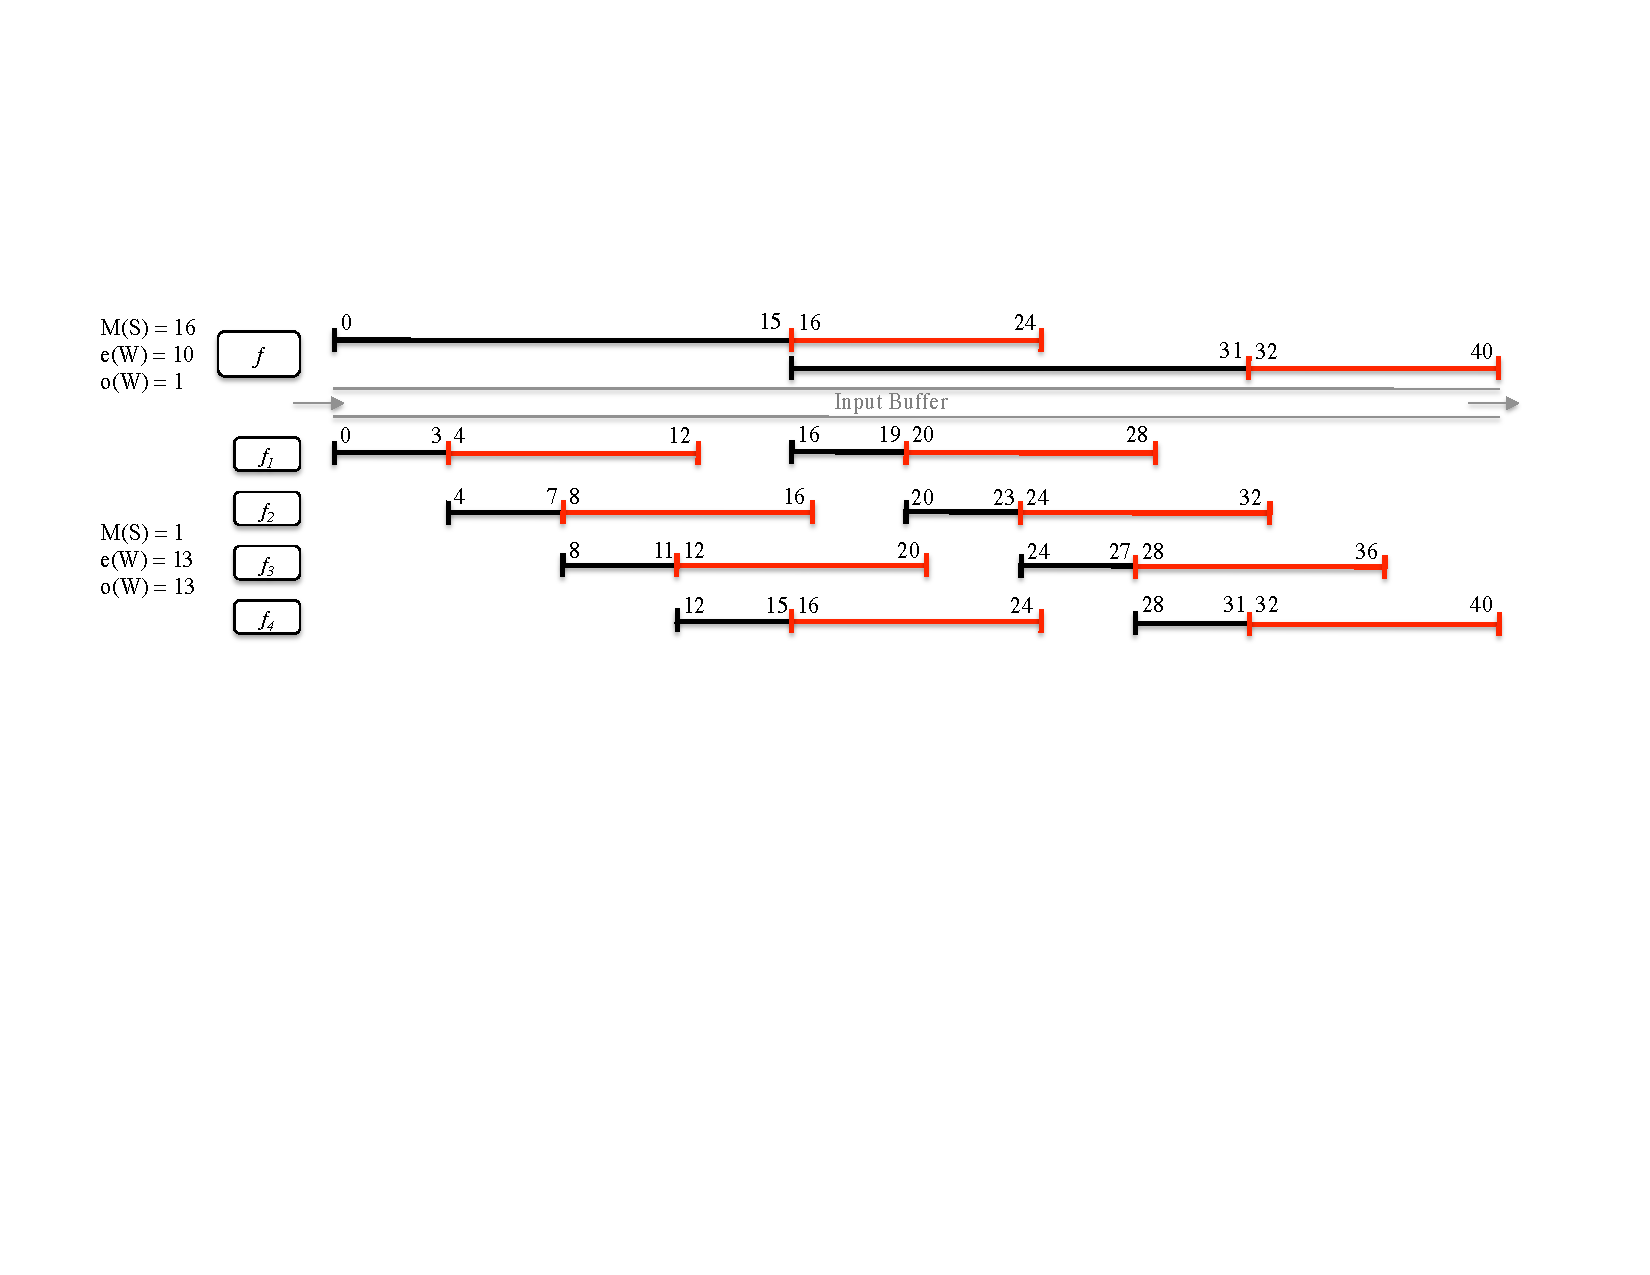
\includegraphics[width=3.0in]{figures/fission-sharing.pdf}
\caption[An example of the sharing required by fission.]  { An
  example of the duplication of items required by fission.  Filter $f$
  is fissed by 4 into $f_1$ - $f_4$.  Two steady-states of the item
  indices required for both $f$ and the fission products are shown.
  Item indices that are inspected but not dequeued are in red.  For the
  fission products, it is required to duplicate 1 out of 4 items to
  all 4 filters, and the remaining 3 items are duplicated to 3
  filters.  Notice that the number of items inspected by the fission
  products is the same as $f$, but the total number of items dequeued 
per steady-state is split across the $f_i$s.
\label{fig:fission-sharing}}
\end{figure}

Data parallelization is possible if the compiler can reason about the
sharing requirement of the sliding window filter.  When a sliding
window filter is parallelized via the process of fission, the window
state inherent between iterations is transformed into the
communication of shared items to multiple products of the filter.
Figure~\ref{fig:fission-sharing} gives an example of the sharing
requirement between fission products for a fission application. 
Previous work implement fission of sliding window filters via
duplication of all input items to all fission products and decimation
of unneeded items at each product filter~\cite{streamit-asplos}.  We
call this technique {\it DupDec}. If each product is mapped to a
distinct core, the replication of items is achieved via the
communication network.

The efficiency of DupDec depends on the application being mapped and
the communication mechanism of the target. For our benchmarks, we can
determine what percentage of total steady-state communication is
unnecessarily duplicated by DupDec guided by the techniques described
in~\cite{gordon-asplos06}:

\begin{itemize}
\item ChannelVocoder: 38\% unnecessarily duplicated (5,200 of 13,336
      total items)
\item FMRadio: 61\% unnecessarily duplicated (1,108 of
      1,808 total items) 
\item FilterBank: 0\% duplicated (912 total items)
\end{itemize}

Our techniques will always avoid unncessary duplication of input
items.  Even without unnecessarily duplication of items, inter-core
communication as a result of fission accounts for a large percentage
of the total items communicated between filters of an application.
ChannelVocoder has 48\% of total communication as inter-core
communication caused by fission, Filterbank 50\%, and FMRadio 93\%.
Employing our techniques, for our benchmarks, we are able to reduce
the percentage of inter-core communication by altering the steady
state.

In the general case, when fissing a filter that peeks, i.e., a filter
$f$ with $e(W, f) - o(W, f) = \mt{dup}_f < C(f) > 0$, by $P$, the producers
of $f$ need to duplicate output items to an average of:

\[ \max \left ( 1 + \frac{C(f)}{M(S, f) \cdot o(W, f) / P}, P \right )\]

\noindent fission products of $f$.  Figure~\ref{fig:fission-sharing}
gives an example of the required sharing for a fission application.
The filter $f$ is duplicated 4 ways, has $C(f) = 9$, $o(W, F) = 4$,
and $M(S, f) = 16$.  From the above formula, each item is duplicated
to an average of $3.25$ fission products.

\section{Filter Fission}

This section covers an improved form of fission applied to nodes of the
general graph.  Applying fission to nodes of the general graph allows
the compiler to express more precise communication patterns for the
distribution of input items to the fission products.  This allows the
fission technique to avoid unnecessary duplication (and thus
communication) of input items.  Figure~\ref{fig:fission-versus}
demonstrates an example of the savings in communication for fission on
the general graph versus fission on the StreamIt graph.

A key design goal for the implementation of fission on the general graph
was that communication between levels of the stream graph be efficient
(see Section~\ref{sec:levels} for the description of a level).  Often
when data parallelism is applied, the producer filters in level $l$ are
fissed at the same width as the consumer filters in level $l + 1$.  To
make this common case efficient, general graph fission communicates a
large number of items between disjoint producer-consumer pairs from the
levels.  Next, a small number of items (the number of items inspected by
the consumer filter) is duplicated and communicated from consumer to a
producer in a different pair.  Figure~\ref{fig:fission-versus}(c),
demonstrates this pattern, with $u_i$ and $v_i$ forming the pairs.  Each
pair should be mapped to the same core, so that the bulk of
communication for the fission distribution pattern is intra-core.  For
Figure~\ref{fig:fission-versus}(c), if the pairs are mapped to same
core, only 3 of 12 items are communicated inter-core.


In the general case, when fissing a filter that peeks, i.e., a filter
$f$ with $e(W, f) - o(W, f) = \mt{dup}_f < C(f) > 0$, by $P$, the producers
of $f$ need to duplicate output items to an average of:

\[ \max \left ( 1 + \frac{C(f)}{M(S, f) \cdot o(W, f) / P}, P \right )\]

\noindent fission products of $f$.  Figure~\ref{fig:fission-sharing}
gives an example of the required sharing for a fission application.
The filter $f$ is duplicated 4 ways, has $C(f) = 9$, $o(W, F) = 4$,
and $M(S, f) = 16$.  From the above formula, each item is duplicated
to an average of $3.25$ fission products.

Before we describe the fission transformation, we need to list the
preconditions that must hold before fission of $f$ by $P$ in the general
graph can be performed:
\begin{itemize}
\item $C(f) < (M(S,f) / P) \cdot o(W, f)$. The items remaining of
  the input buffer of the original filter after initialization must be
  less than the number of items dequeued by each fission product.
  This implies $\mt{dup}_f < (M(S,f) / P) \cdot o(W, f)$ since
  $\mt{dup}_f \le C(f)$.  If $\mt{dup}_f$ for the steady-state is greater
  than the number of items that each fission product pops, then some
  items will be duplicated to more than 2 fission products.  We do not
  support this case, as it can be avoided, and we want to limit
  inter-core communication.

\item $M(S,f) \mod P = 0$. In this version of the algorithm we create
  fission products with equal work, an equal division of the original
  steady-state multiplicity of $f$.  This restriction can be relaxed
  via simple modifications to the algorithm.
\end{itemize}
\noindent All the multiplicities of the steady-state can be multiplied
by the same constant $c$, and the result will still be a valid
steady-state.  We call this process {\it increasing} the steady-state
of the graph by $c$.  Each of these preconditions can be enforced by
increasing the steady-state of the graph.


\begin{figure*}
\centering
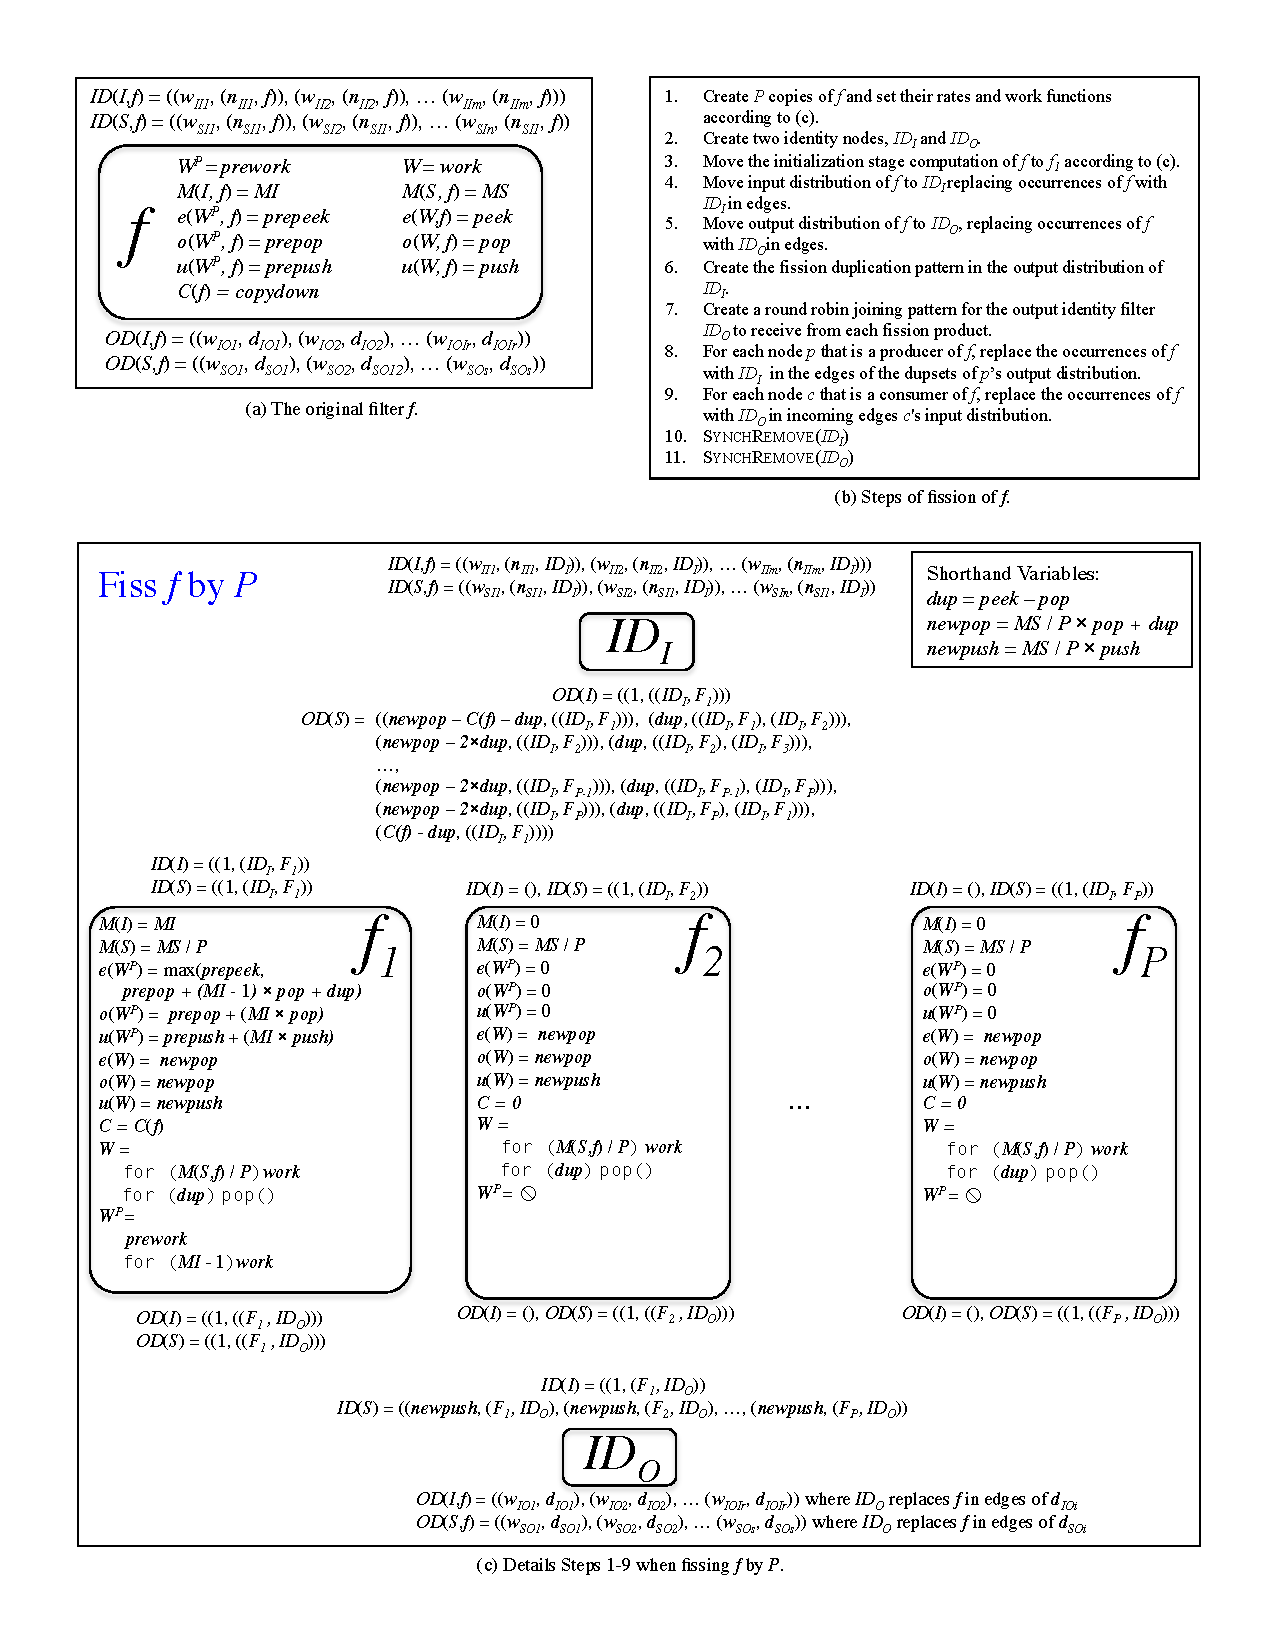
\includegraphics[width=\textwidth]{figures/general-fission.pdf}
\caption[Fission of a node in the general stream graph.]{Fission of a
  node $f$ by $P$ in the general stream
  graph.\label{fig:general-fission}}
\end{figure*}

The details of fission on a filter of the general stream graph are
given in Figure~\ref{fig:general-fission}.  The process includes the
following steps (Figure~\ref{fig:general-fission} illustrates steps
1-9): 
\begin{enumerate}
\item Create $P$ copies of $f$ and set their rates
and work functions according to Figure~\ref{fig:general-fission}.
\item Create two identity nodes, $ID_I$ and $ID_O$, that will encode
  the distribution for the fission.
\item Move the initialization stage computation of $f$ to $f_1$
  according to Figure~\ref{fig:general-fission}. 
\item Move input distribution of $f$ to $ID_I$
replacing occurrences of $f$ with $ID_I$ in edges.
\item Move output distribution of $f$ to $ID_O$, replacing
occurrences of $f$ with $ID_O$ in edges.
\item Create the fission duplication pattern in the
output distribution of $ID_I$.
\item Create a round robin joining pattern for the output identity
  filter $ID_O$ to receive from each fission product.
\item For each node $p$ that is a producer of $f$, replace the
 occurrences of $f$ with $O_I$ in the edges of the dupsets of $p$'s
 output distribution.
\item For each node $c$ that is a consumer of $f$, replace the
 occurrences of $f$ with $O_O$ in incoming edges $c$'s input
 distribution.
\item \textsc{SynchRemove}($ID_I$)
\item \textsc{SynchRemove}($ID_O$)
\end{enumerate}

To understand the transformation, we first need to understand the item
distribution and sharing that is required by fission on a filter $f$
that adheres to the preconditions above.
Figure~\ref{fig:fission-sharing2} gives another example of the input
items required by fission products.  In this example, both:

\[ C(f) = \mt{dup}_f < (M(S,f) / p) \cdot o(W, f) \]
\[ M(S, f) \mod P = 0\]

\noindent so $f$ adheres to the preconditions stipulated above for
general fission.  In the example, the items read for $f$ plus its
fission products for $P=4$ are shown for the initialization plus two
steady-states.  After the initialization stage, $C(f) = 2$ items are
enqueued to the input buffer by the producer(s) to $f$, and $M(S,f)
\cdot o(W, f) = 16$ items are enqueued by the producer(s) for each
steady-state.  Examining the sharing requirement for fission products of
the second steady-state, we can see a pattern emerge with the following
features:

\begin{itemize}
\item No item is read by more than 2 fission products.
\item  A fission product does not need to remember items across
  steady-state executions of itself.
\item Only the first fission product $f_1$ is required to receive the $C(f)$
  initialization  items because $C(F) < (M(S,f) / p) \cdot o(W, f)$,
  and it will consume the $C(f)$ items on its first invocation.
\item The presence of the $C(f)$ items in the input buffer after
  initialization must be accounted for by shifting the read pattern
  for the fission products.  The first fission product $f_1$ is offset by
  $C(f)$ items in that it reads its first $C(f)$ items from the
  previous execution stage.  In the steady-state, $f_1$ executing at
  steady-state iteration $i$ shares items with $f_P$ executing at
  steady-state iteration $i-1$.
\end{itemize}


\begin{figure*}
\centering
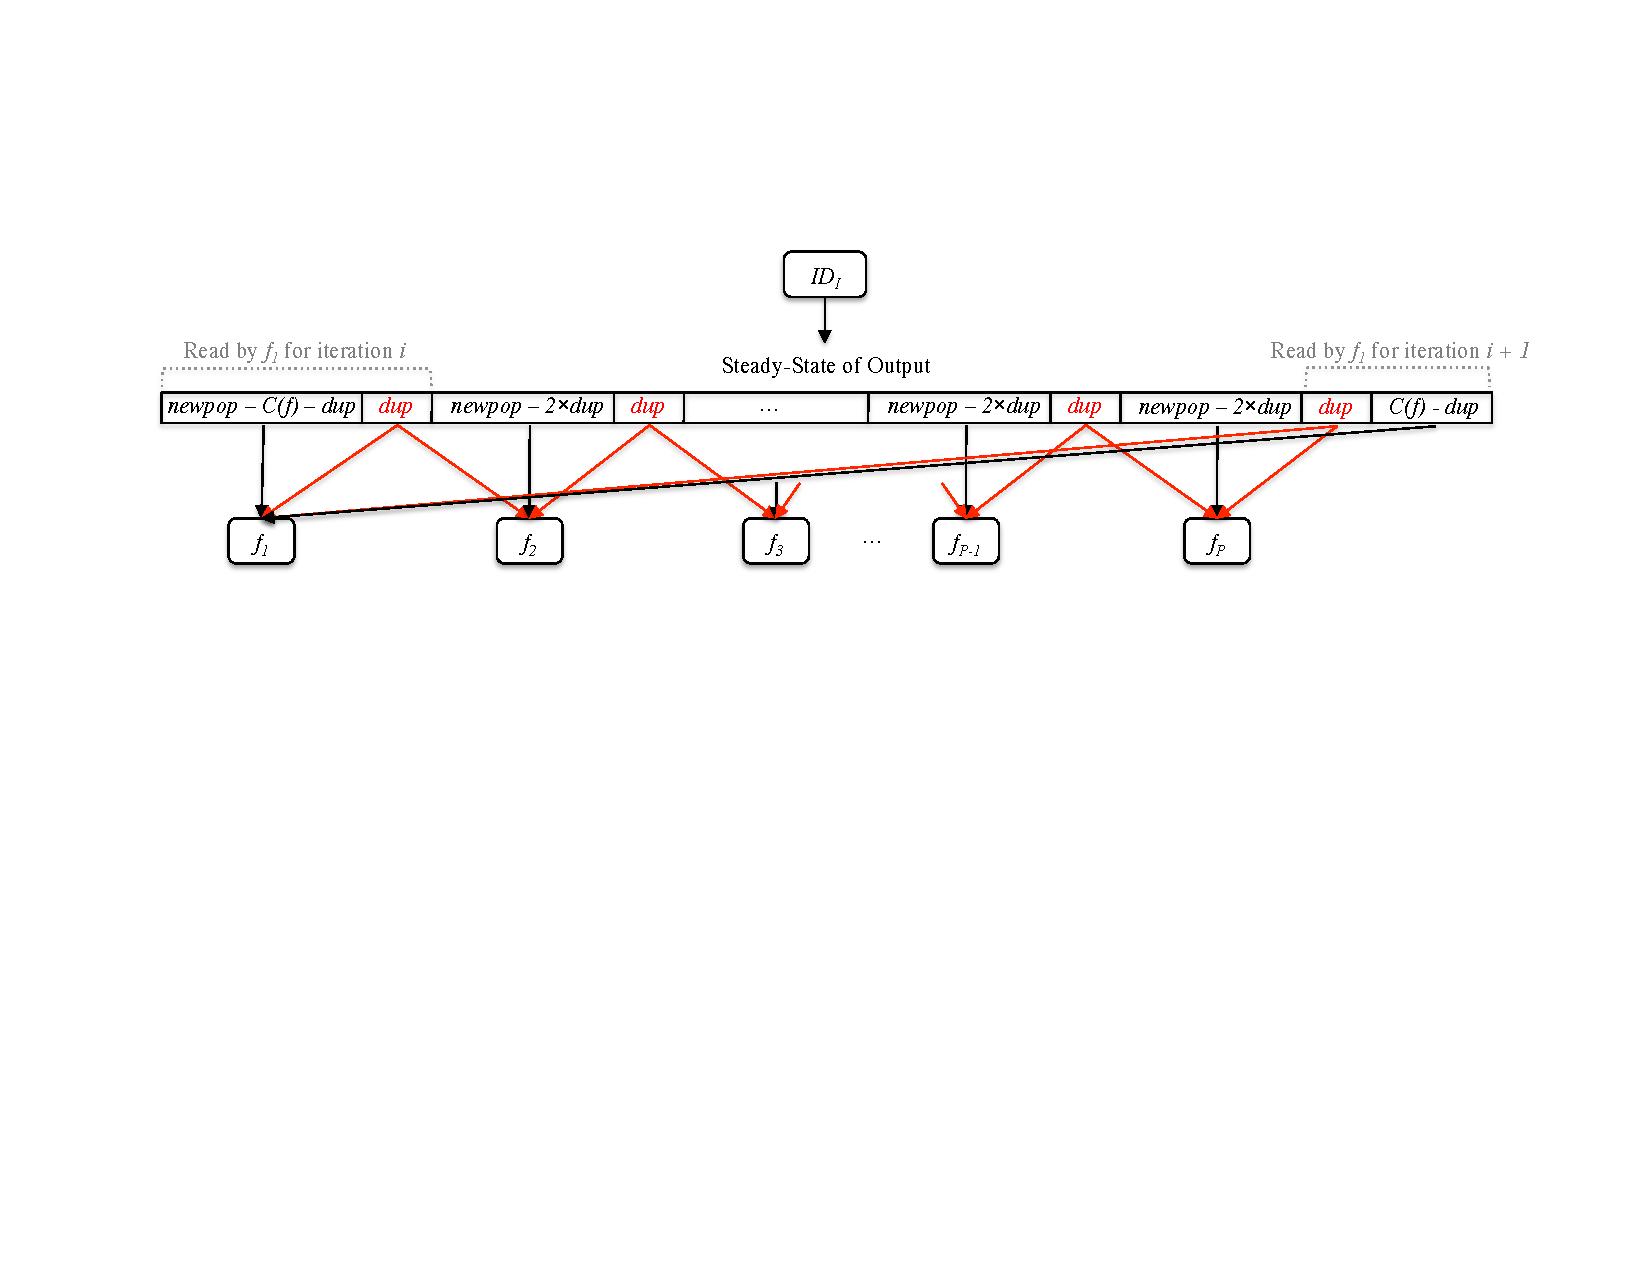
\includegraphics[width=\textwidth]{figures/split-pattern.pdf}
\caption[The output distribution required for general
fission.]{
The steady-state output distribution installed for identity node
$ID_I$ by general fission.  Red edges denote items that are shared
across fission products via duplication.  Though not demonstrated in
the example of Figure~\ref{fig:fission-sharing2}, in the general
case, if $C(f) > dup$, $C(f) - dup$ items at the end of the
steady-state input are distributed to $f_1$. \label{fig:split-pattern}}
\end{figure*}

The general fission transformation creates two identity nodes ($ID_I$
and $ID_O$) that are encoded to implemented the data distribution for
the fission products.  The pattern seen in
Figure~\ref{fig:fission-sharing2} and described above is common to the
transformation for all filters we seek to fiss that meet the
preconditions of the transformation.  This sharing pattern is encoded
in the output distribution pattern for the identity filter $ID_I$.
Figure~\ref{fig:split-pattern} shows the weights for the output
distribution and how these weights are distributed to the fission
products.

The input distribution of $ID_I$ is set to the input distribution of
$f$.  Thus, $ID_I$ joins data as described by $f$'s input
distribution, and splits data according to the fission output pattern
for sharing between at most 2 filters.  The output identity $ID_O$
collects the output items of the fission products in a weighted round
robin, and the distributes them according to $f$'s output distribution.

Since a fission product, does not need to remember items across
firing, a fission product's peek rate equals its pop rate in the
steady-state.  This rate equals the division of $f$'s dequeued
items plus the number of items inspected but not dequeued by $f$ for
each firing:   

\[ o(S,f_i) = e(S, f_i) = \frac{M(S, f)}{P} \cdot o(W, f) + \mt{dup} \]

\noindent The peeking of the original filter $f$ is now encoded in
the sharing across fission products achieved via the duplication
pattern.

The computation and communication performed by $f$ during the
initialization stage is transferred completely to the first fission
product, $f_1$.  Since, by construction, only $f_1$ requires the items
remaining after the initialization stage.  The other fission products
are idle during this stage.

The final steps of the general fission transformation applies
\textsc{SynchRemove} to remove the identity filters, and stitch the
communication directly between the fission products and $f$'s
producer(s) and consumer(s).

%\section{Data Parallelization Common Case}

% The techniques covered above are employed during the compiler flow
% outlined in Chapter~\ref{ch:datapar} to effectively leverage data and
% task parallelism.  The coarsened StreamIt graph is converted into a
% general by employing \textsc{SynchRemove} (see
% Section~\ref{sec:synch-remove} for details).  \textsc{JudiciousFission} is
% performed on the coarsened general graph using the technique covered
% in Section~\ref{sec:levels}.  Fission of a node in the general graph
% replaces fission of a filter in the StreamIt graph (see
% Section~\ref{sec:fission-streamit}) in the process of judicious
% fission.  Conversion to the general graph with synchronization
% removal, accompanied by employing general fission, greatly reduces the
% inter-core communication requirement of the resulting mapping when
% fissing filters that peek.  Figure~\ref{fig:fission-versus} gives a
% simple example of the potential savings.

% The design of the general fission algorithm was informed by the fact
% that for most fission applications of judicious fission, a producer
% and consumer are fissed by an equal width.  This is because in most of
% our benchmarks, a level's width of task parallelism is equal to the
% width of task parallelism for it's consuming level.  In this case,
% fission on the general graph will map the bulk of communication to
% intra-core resources.  Furthermore, in the next section we demonstrate
% that the ratio of inter-core communication to total communication is
% parametrizable for this case.

To understand why general fission achieves the reduction of inter-core
communication for this case, we must remember a few properties of the
steady-state schedule of the stream graph.  For single output producer
$f$ and single input consumer $g$, where $(f,g) \in E$:

\[ M(S, f) \cdot u(W, f) = M(S,g) \cdot o(W,g) \]

\noindent When $f$ and $g$ are fissed (employing general fission) by
the same amount $P$, the above equality no longer holds across all the
fission products if $g$ peeks.  This is because the peeking of $g$ is
converted into duplication of items to the products of $g$'s fission
application.  The fission products of $g$ each consumes more items
than each fission product of $f$ produces.  However, we can make it
the case that {\it most} of the outputs of a fission product $f_i$ are
directed to $g_i$, for each $1 \le i \le P$.  When each $f_i$ and
$g_i$ are mapped to the same core, the bulk of communication is
intra-core.

\begin{figure*}[t]
\centering
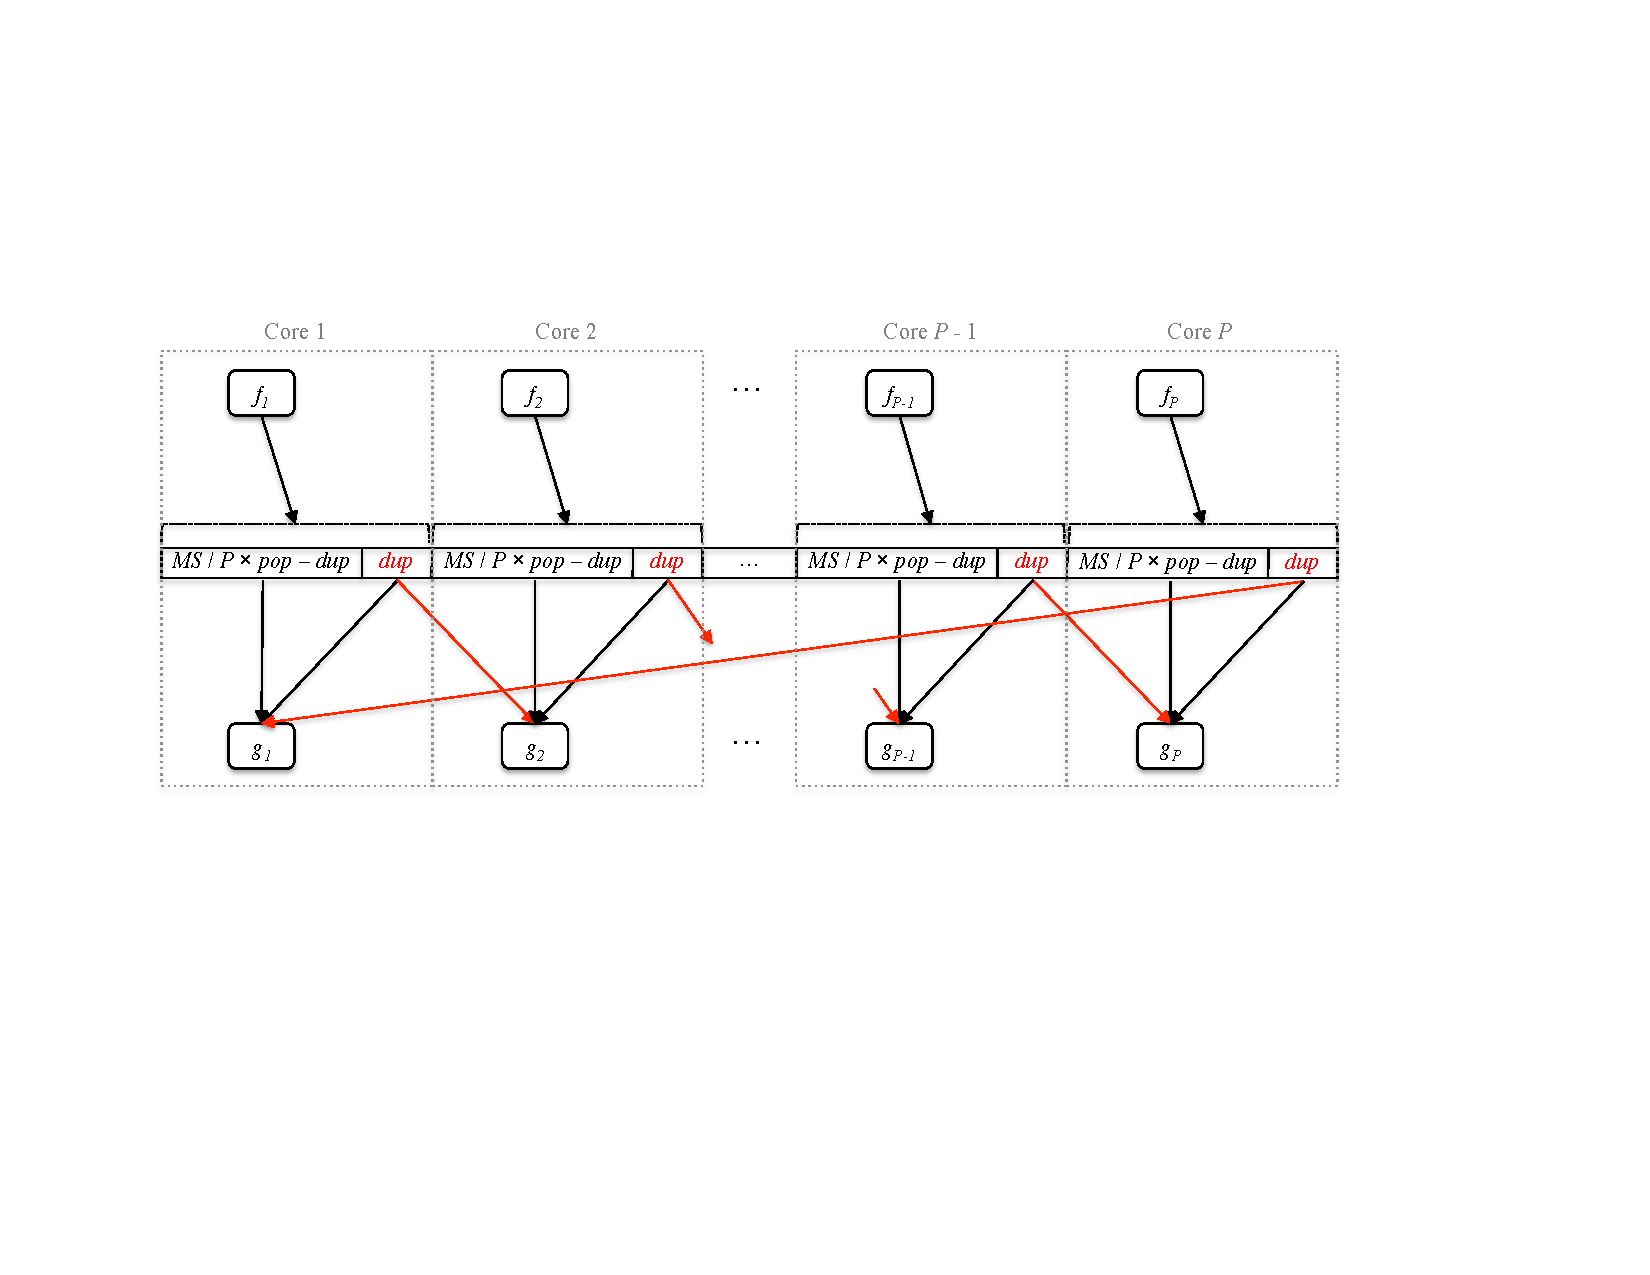
\includegraphics[width=6in]{figures/core-comm.pdf}
\caption[Communication between cores for fission of producer and
consumer.]{ Communication details for fission products of consumer $f$
  and producer $g$ each fissed by $P$.  $f$ was a single output node,
  and $g$ was a single input node.  Furthermore, $C(g) = \mt{dup}_g$.
  Each $f_i$, $g_i$ pair are mapped to the same core.
  The sizes of the buffer sections are in terms of $g$. Red arrows
  denote inter-core communication. \label{fig:core-comm}}
\end{figure*}

Figure~\ref{fig:core-comm} illustrates the details of communication
between $f$ and $g$ when each is fissed by $P$.  In the figure it is
assumed that $C(g) = \mt{dup}_g $, meaning the number of items
remaining after the initialization schedule equals the number of items
that $g$ inspected but did not pop.  Each $f_i$ produces $M(S,f)/p
\cdot u(S,f)$ items, while each $g_i$ must consume the original pop
rate multiplied by it's slice of $f$'s multiplicity plus the number of
inspected items of $g$:

\[ M(S,g)/P \cdot o(W, g) + C(g) \]

\noindent Since $M(S,g)/P \cdot o(W, g) = M(S,f)/p
\cdot u(S,f)$, the number of items each $f_i$ produces and the number
of items each $g_i$ consumes differs by $C(g)$.
As Figure~\ref{fig:core-comm} demonstrates, each $g_i$
receives $C(g)$ duplicated items from $g_{i-1}$ (with $g_1$
receiving from $f_p$).  When the fission products are assigned to
cores as given in the figure, the percentage of inter-core
communication to total communication can be reduced to:

\begin{equation}
\label{eq:min-dup}
\mt{InterCore}(g) = \frac{C(g)}{M(S,g) / P * o(W, g)}
\end{equation}

\noindent This percentage corresponds to the best case, in which a
producer and consume are fissed by the same amount and $C(g) =
\mt{dup}_g$.  This case is common in our benchmarks.

The next section covers a technique that seeks to decrease the percentage
of total communication that must be communicated inter-core.  The
technique directly decreases the number of items that are shared,
while also increasing the alignment of communication to minimize
inter-core communication.

\section{Sharing Reduction}

A key design goal for the implementation of fission was that
communication between producers and consumers of the stream graph be
efficient.  Often when data parallelism is applied, the producer
filter is fissed by the same factor as the consumer filter.  To make
this common case efficient, general graph fission communicates a large
number of items between disjoint producer-consumer pairs of products
of the fission.  Next, a small number of items (the number of items
inspected by the consumer filter) is duplicated and communicated from
producer to a consumer in a different pair.

Figure~\ref{fig:remaining-dup} illustrates the details of
communication between $f$ and $g$ when each is fissed by $P$ with each
$f_i$ mapped to a distinct core, and to the same core as $g_i$.  From
the figure, notice that $C(g)$ items are communicated from $f_i$ to
$g_{i+ 1}$, with $f_P$ sending to $g_1$.  Of the $C(g)$ items,
$\mt{dup}_g$ items are required by both $g_i$ and $g_{i+1}$.  This
corresponds to the orignal number of input items of $g$ that were
inspected but not dequeued for one firing of $g$.  The remaining items,
$C(g) - \mt{dup}_g$, are required to be transfered from $f_i$ to
$g_{i+1}$ when $C(g) > \mt{dup}$ because of misalignment of the items
produced by $f_i$ and required by $g_i$.

When the fission products are assigned to
cores as given in the figure, the percentage of inter-core
communication to total communication can be quantified as:
{\ninepoint
\begin{equation}
%b\vspace{-2pt}
\label{eq:min-dup}
\mt{InterCore}(g) = \frac{C(g)}{M(S,g) / P * o(W, g)}
%\vspace{-4pt}
\end{equation}
}
\noindent This percentage corresponds to inter-core communication
ratio for each product filter and, since all product filters have the
same rates, for the total inter-core communication required for the
fission of $g$.

This section covers a technique that seeks to decrease the percentage
of total communication that must be communicated inter-core.  The
technique directly decreases the number of items that are shared,
while also increasing the alignment of communication to minimize
inter-core communication.

Since streaming applications typically execute for many iterations of
the steady-state, it is legal to increase the steady state by $c$.  As
long as this constant $c$ is less than the number of steady-state
iterations $I$ of the application, and $c$ is a factor of $I$.


\begin{figure*}[t]
\centering
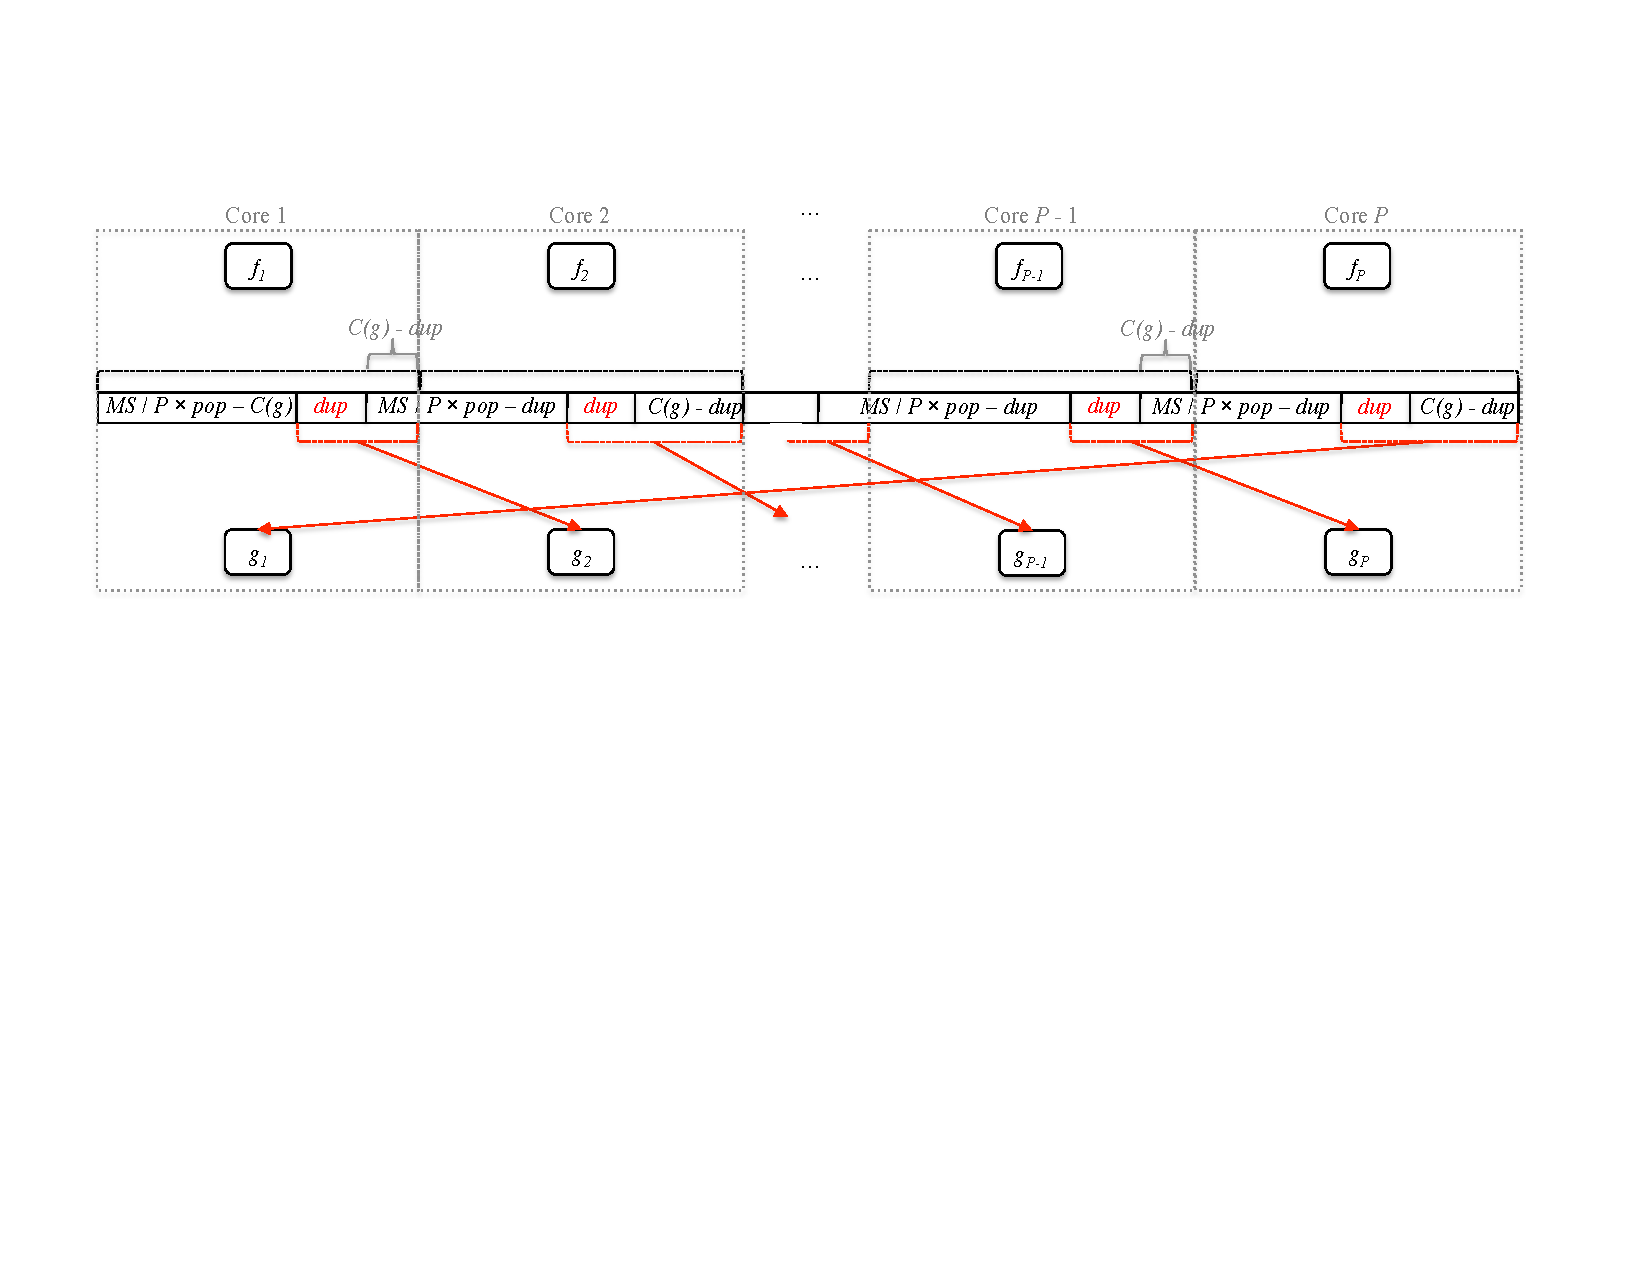
\includegraphics[width=6in]{figures/remaining-dup-case.pdf}
\caption[Extra inter-core communication when $C(g) > \mt{dup}_g$.]
{Fission products of consumer $f$
  and producer $g$ each fissed by $P$.  $f$ was a single output node,
  and $g$ was a single input node.  For $g$, $C(g) > \mt{dup}_g$.
  Each $f_i$, $g_i$ pair is mapped to the same core.  The sizes of
  the buffer sections are in terms of $g$. Red arrows denote
  inter-core communication.  \label{fig:remaining-dup}}
\end{figure*}


By recognizing this property, we can directly reduce the amount of
inter-core communication that occurs between the fission products of a
fissed peeking filter for many cases of general fission, including the
common case.  In Equation~\ref{eq:min-dup} we can directly control the
steady-state multiplicity of $g$, $M(S,g)$.  We can calculate a
constant $c_g$ such that the percentage is less than a threshold
$T_{\mt{sharing}}$:
{\ninepoint
\begin{equation}
\label{eq:ic-thresh}
c_g = \frac{1}{T_{\mt{sharing}}} \cdot \frac{C(g) \cdot P}{M(S,g) \cdot o(W,g)}
\end{equation}
}
\noindent where $0.0 < T_{\mt{sharing}} \le
\mt{InterCore(g)}$. Increasing the steady-state of the graph by $c_g$
before general fission is applied will assure that the percentage of
items duplicated will be equal to $T_{\mt{sharing}}$.  Sharing
reduction works by increasing the ratio of number of items that are
only needed by one product to the number of items that are needed by
two products.  When we increase the steady-state, in
Figure~\ref{fig:remaining-dup}, the shared (red) sections of the input
buffer to $g$ remain fixed in size, while the private sections of the
input buffer (black) grow.

\subsection{Sharing Reduction for Other Fission Cases}

The sharing reduction optimization does not apply as simply to all
cases of fission of a peeking filter.  Consider the case where we have
single output producer $f$ and single input consumer $g$ with $(f,g)
\in E$, but $f$ and $g$ are fissed by differing widths, i.e., $P_f \ne
P_g$.  This case engenders inter-core communication not only because
of sharing but because of the communication required by the differing
fission widths.  

Going forward, let us assume that $P_f > P_g$.  If $P_f$ is a multiple
of $P_g$, the analysis is straightforward: the percentage of
inter-core communication to total communication is $(1 -
\frac{P_g}{P_f}$). If $P_f$ is not a multiple of $P_g$ misalignment
also occurs because for one or more $g_j$, it's input does not begin
in alignment with any $f_i$'s.  The analysis of the percent of
inter-core communication for this latter case is complex, but it
suffices for our purposes to bound it by $(1 - \frac{P_g}{P_f})$.

Also consider the case where $g$ has multiple inputs. In this case $g$
receives $\mt{RI}(f, g, S) \cdot M(S, g) \cdot o(W,g)$ items from $f$
during the steady-state, and $(1 -\mt{RI}(f, g, S) \cdot M(S, g) \cdot
o(W,g))$ from its other producers. There is a choice: for which
producer of $g$ to optimize the communication of $g$? If $f$ is
chosen, then the assignment of filters to cores should minimize the
inter-core communication by co-locating the fission products of $f$
and $g$ just as the assignment would when $g$ is single input.
However, the calculation must now account for the inter-core
communication of the other producers sending to the fission products
of $g$. 

Now, considering both cases above, we define $\mt{InterCore}(g, f)$ to
approximate the percentage of inter-core communication to total
communication for the input of the fission products of $g$ optimizing
for the placement of the fission products of $f$:
{\ninepoint
\begin{equation}
\label{eq:tcomm-fopt}
 \mt{InterCore}(g, f)   =  (1 -\mt{RI}(f,g, S) \cdot \frac{P_g}{P_f})
 + \frac{P_g \cdot C(g)}{M(S, g) \cdot o(W, g)}
\end{equation}
}
\noindent The first term approximates the inter-core communication due
to (i) the fission factor discrepancy between $f$ and $g$, and (ii) the
multiple inputs of $g$.  The second term quantifies the percentage of
inter-core communication caused by the sharing due to peeking.

Increasing the steady-state will not alter the first term of
Eq.~\ref{eq:tcomm-fopt}.  However, the second term can be reduced
because a smaller percentage of steady-state items needs to be
duplicated.  By Amdahl's law, increasing the steady-state can only
decrease $\mt{InterCore}(g, f)$ to under $T_{\mt{sharing}}$ if the
second term of Equation~\ref{eq:tcomm-fopt} accounts for more than
$(1-T_{\mt{sharing}} )$ of the duplication.  

We need to prevent the application of increasing the steady-state to a
filter $g$ that will not benefit from it because the majority of
inter-core communication from fission of $g$ is not caused by $g$'s
sliding window.  We define a constant $T_{\mt{apply}}$ such that
sharing reduction should only be applied to $g$ optimizing for $f$ if:
{\ninepoint
\begin{equation}
\label{eq:apply-sharing}
T_{\mt{sharing}}  >  T_{\mt{apply}} \ge (1 -\mt{RI}(f,g, S) \cdot
\min(\frac{P_g}{P_f}, \frac{P_f}{P_g}))
\end{equation}
}
% \begin{equation}
% T_{\mt{sharing}}  >  T_{\mt{apply}} \ge (1 -\mt{RI}(f,g, S) \cdot
% \frac{P_g}{P_f})
% \end{equation}

\noindent Since it was first assumed that $P_f > P_g$, in order to
generalize we must choose the appropriate fraction of local
communication by taking the minimum of the two fission width ratios.

In the common case where $f$ and $g$ are fissed by the same width, and
$f$ has single output and $g$ has single input, the RHS of
Eq.~\ref{eq:apply-sharing} evaluates to 0, indicating to always apply
sharing reduction.  If however, the RHS of Eq.~\ref{eq:apply-sharing}
does not evaluate to 0, there exists inter-core communication that is
not attributed to sliding windows.  In this latter case,
$T_{\mt{apply}}$ determines at what percent of total inter-core
communication, non-sliding-window inter-core communication should
prevent the application of sharing reduction.  For example, if
$T_{\mt{apply}} = .05$, then we will apply sharing reduction only when
sliding window inter-core communication accounts or at least 95\% of
total inter-core communication for the proposed fission application of
$g$. $T_{\mt{apply}}$ prevents the application of sharing reduction to
fission when the bulk of inter-core communication of the fission is
not caused by sliding windows, and thus will not be reduced by
increasing the steady-state.

% For simplicity of analysis, let us assume that $C(g)
% = 0$, and $P_f$ is a multiple of $P_g$. Figure~\ref{fig:diff-widths}
% presents an example with these assumptions.  In the example, $f$ and
% $g$ are fissed by 8 and 4 respectively.  Since we want to maintain
% data parallelism, each $f_i$, $1 \le i \le P_f$, is mapped to a
% distinct core, as is each $g_j$, $1 \le j \le P_g$.  Since each $f_i$
% produces half the number of items required by each $g_j$, half the
% communication in this case is inter-core, caused by the misalignment
% of the rates of the producer and consumer fission products.


% Additionally, if $C(g) > 0$, it is required to share $C(g)$ items
% between two cores.  There are $P_g$ sections of $C(g)$ items, and this
% data has to be communicated inter-core to one other core.  Given this
% analysis, we can quantify an {\it approximation} of the percentage of
% inter-core communication for the fission application of $g$ when $P_f
% > P_g$:

% \begin{align}
% \mt{InterCore}(g) & = & \frac{(1 - \frac{P_g}{P_f}) \cdot M(S, g) \cdot o(W, g) +
% P_g \cdot C(g)}{M(S, g) \cdot o(W, g)} \\
% \label{eq:diff-fiss}
% \mt{InterCore}(g) & = & (1 - \frac{P_g}{P_f}) +
% \frac{P_g \cdot C(g)}{M(S, g) \cdot o(W, g)}
% \end{align}

% The first term on the RHS of Equation~\ref{eq:diff-fiss} gives the
% percentage of inter-core communication produced by the fission width
% inequality.  

% \begin{equation}
% \label{eq:tcomm-fopt1}
%  \mt{InterCore}(g,f)   = (1 - \mt{RI}(f,
%    g, S))  + (1 - \frac{P_g}{P_f}) \cdot \mt{RI}(f,
%    g, S)   + \frac{P_g \cdot C(g)}{M(S, g) \cdot o(W, g)} 
% \end{equation}

% \noindent The first term accounts for the percentage of items that $g$'s fission
% products receive from producers that are not products of $f$.  The
% second term, the percentage items that are communicated inter-core
% because of the fission width mis-alignment, must now account for the
% fact that not all items are from $f$.  Equation~\ref{eq:tcomm-fopt1}
% can be simplified to:


\subsection{Sharing Reduction Applied to the Stream Graph}
So far we have considered the application of the sharing reduction
optimization to a single filter $g$ in the stream graph.  Now we will
cover how to apply sharing reduction across all the filters of the
stream graph for which it is appropriate.  The goal is reduce the
percentage of inter-core communication due to the sharing between
fission products of all peeking filters to {\it approximately}
$T_{\mt{sharing}}$ of total inter-core communication for the fission
of all peeking filters.  Sharing reduction may not achieve
$T_{\mt{sharing}}$ because there may exist peeking filters that are to
be fissed for which Equation~\ref{eq:apply-sharing} cannot be
satisfied.  For these filters, we do not apply the sharing reduction
optimization.

The process of applying sharing reduction to the entire stream graph
consists of determining which filters are appropriate and determining
a steady-state multiplier by which to increase the graph.  To
determine the steady-state graph multiplier, the compiler calculates
the percentage of sharing over all of the filters which adhere to
Equation~\ref{eq:apply-sharing}.  Let $\Phi$ denote the set of filters
for which Equation~\ref{eq:apply-sharing} holds and that we seek to
fiss:
{\ninepoint
\begin{equation}
\label{eq:sr-mult}
c = \frac{1}{T_{\mt{sharing}}} \cdot \frac{\sum_{g \in \Phi} P_g \cdot C(g) }{\sum _{g \in
    \Phi} M(S, g) \cdot o(W, g)}
\end{equation}
}
\noindent Increasing the steady-state by $c$ for all filters of the
graph will reduce the total sharing for the filters of $\Phi$ to
$T_{\mt{sharing}}$.  




% In the
%  graph before fission is applied, $C(g)$ items will remain in the
%  input buffer of $g$ between steady-state iterations.  After fission by $P$,
%  for each steady-state, $g_1$ will first consume the $C(g)$ items that
%  $f_p$ sent it from the previous steady-state iteration.  $g_1$ will
%  then require:

% \[ M(S, g)/P \cdot o(W, g) + \mt{dup} - C(g)\]

% \noindent additional items from $f_1$.\footnote{It is guaranteed that
%   $M(S, g)/P \cdot o(W, g) > C(g)$ by the precondition of general
%   fission.} This requirement is less than the number of items that
% $f_1$ produces $M(S, g)/P \cdot o(W, g)$ since $C(g) > \mt{dup}$. So,
% $C(g) - \mt{dup}$ items must be transferred from $f_1$ to $g_2$ in
% addition to the shared and duplicated $\mt{dup}$. In all, $C(g)$ items
% must be transferred from $f_i$ to $g_{i+1}$.

%  Each $f_i$ produces $M(S,f)/p
% \cdot u(S,f)$ items, while each $g_i$ must consume the original pop
% rate multiplied by it's slice of $f$'s multiplicity plus the number of
% inspected items of $g$:

% \[ M(S,g)/P \cdot o(W, g) + C(g) \]

% \noindent Since $M(S,g)/P \cdot o(W, g) = M(S,f)/p
% \cdot u(S,f)$, the number of items each $f_i$ produces and the number
% of items each $g_i$ consumes differs by $C(g)$.
% As Figure~\ref{fig:core-comm} demonstrates, each $g_i$
% receives $C(g)$ duplicated items from $g_{i-1}$ (with $g_1$
% receiving from $f_p$).  

\section{Data Parallelization of Stream Graph}


General fission and sharing reduction are employed after
\textsc{JudiciousFission} (see Algorithm~\ref{alg:jd}) calculates a
fission width for each filter of the graph.  The formulation of
general fission in Section~\ref{sec:general-fission} includes two
preconditions for filter $g$:

\begin{equation}
\label{eq:fiss-precond1}
C(g) < (M(S,g) / P) \cdot o(W, g) 
\end{equation}
\begin{equation}
\label{eq:mod-fiss}
M(S,g) \mod P = 0
\end{equation}

\noindent The compiler is required to calculate a multiplication
factor $c$ for the entire graph that satisfies the preconditions for
every filter.  At the same time, $c$ applies sharing
reduction to the graph by increasing the graph such that
Equation~\ref{eq:sr-mult} is satisfied by the constant.

\textsc{DataParallelize} of Algorithm~\ref{alg:data-parallelize}
highlights the steps for data parallelizing the general graph
representation of the application.  This sequence is applied after the
StreamIt graph has been coarsened and converted to a general graph.
The algorithm first calculates the judicious fission widths for each
filter of the general graph.  For each peeking filter $g$ that will be
fissed, line~\ref{ln:dp1} finds the producer of $g$ that minimizes
Equation~\ref{eq:apply-sharing}.  If this value is below
$T_{\mt{apply}}$, $g$ is added to the sharing reduction calculation by
adding $g$'s shared items and $g$'s total items to the running totals
of each quantity.  Sharing reduction is incorporated into the
steady-state multiplier $\mt{minMult}$ in line~\ref{ln:dp2} employing
Equation~\ref{eq:sr-mult}.  The algorithm applies
Equation~\ref{eq:fiss-precond1} to each peeking filter that will be
fissed by maintain a running value of the minimum multiplier that
enforce the precondition (line~\ref{ln:dp3}).  The sharing reduction
multiplicity ($\mt{minMult}$) is required to be greater than the
precondition multiplier.  Because of the precondition of
Equation~\ref{eq:mod-fiss}, the final multiplication factor for
increasing the steady-state must be a multiple of all the fission
widths calculated by \textsc{JudiciousFission}.  The algorithm assures
this by finding the least common multiple of all the $P_f$'s greater
than $\mt{minMult}$ (line~\ref{ln:dp4}).  The steady-state
multiplicity of the graph is then increased by multiplying all of the
multiplicities by $c$.  Finally, each filter $f$ can be fissed by $P_f$ using
general fission.

\begin{algorithm}[th!]
\caption{Exploit Data Parallelism in the General Graph for $N$ Cores} \label {alg:data-parallelize}
\textsc{DataParallelize}($G = (V, E), N, T_{\mt{sharing}}, T_{\mt{apply}} $)
\begin{algorithmic}[1]
\State $\mt{preCondMult} \gets 1$, $\mt{sharingItems} \gets 0$, $\mt{totalItems} \gets 0$
\State $\triangleright$ For each filter in the graph find the fiss factor
\ForAll {$g \in V$}
\State $P_g \gets $ \Call{JudiciousFission}{$g$, $N$} 
\EndFor
\Statex
\State $\triangleright$ Calculate multiplier for fission preconditions and for sharing reduction
\ForAll {$g \in V$}
\State $\triangleright$ If this is a peeking filter we are fissing:
\If {$P_g > 1 \wedge C(g) > 0$}
\State $\triangleright$ Find the producer of $g$ with the lowest
value for Eq.~\ref{eq:apply-sharing}
\State $f \gets \min_{f \in \mt{In}(g)} (1 -\mt{RI}(f,g, S) \cdot
\min(\frac{P_g}{P_f},\frac{P_f}{P_g} )) $
\label{ln:dp1}
\State $\triangleright$ If the min value is below $T_{\mt{apply}}$,
then record the sharing and total communication
\If {$T_{\mt{apply}} \ge  (1 -\mt{RI}(f,g, S) \cdot
\min(\frac{P_g}{P_f},\frac{P_f}{P_g} ))$}
\State $\mt{sharingItems} \gets \mt{sharingItems} + P_g \cdot C(g)$
\State $\mt{totalItems} \gets \mt{totalItems} + M(S,g) \cdot o(W, g)$
\EndIf 
\State $\triangleright$ Assure that fissing peeking filters adhere to Eq.~\ref{eq:fiss-precond1}
\State $\mt{preCondMult} \gets \max(\mt{preContMult}, \frac{C(g) \cdot P_g}{M(S,g)
 \cdot o(W,g)})$  
\label{ln:dp3}
\EndIf
\EndFor
\Statex
\State $\triangleright$ Find the multiplier for sharing reduction
\State $\mt{minMult} \gets T_{\mt{sharing}} \cdot \frac{\mt{sharingItems}
}{\mt{totalItems}}$
\label{ln:dp2}
\State $\triangleright$ Make sure that multiplier assures all fissing peeking filters
adhere to  Eq.~\ref{eq:fiss-precond1}
\State $\mt{minMult} \gets \max(\mt{minMult}, \mt{preCondMult})$
\State $\triangleright$ Find the least common multiple of the $P_f$'s
greater than $\mt{minMult}$ to adhere to Eq.~\ref{eq:mod-fiss}
\State $c \gets $\Call{LCM}{$\forall P_f | f \in V$} $ >
\mt{minMult}$
\Statex
\label{ln:dp4}
\State $\triangleright$ Increase the steady-state by $c$
\ForAll {$f \in V$}
\State $M(S,f) \gets c \cdot M(S, f)$
\EndFor
\Statex
\State $\triangleright$ Apply general fission to all nodes in the graph
\ForAll {$f \in V$}
\State \Call{GeneralFiss}{$f$, $P_f$}
\EndFor
\end{algorithmic}
\vspace{10pt}
\end{algorithm}


Through empirical experimentation on FMRadio, Filterbank, and
ChannelVocoder, we have settled on $T_{\mt{sharing}} =.10$ and
$T_{\mt{apply}} = 0.05$. These constants are the sweet stop for the two
architectures employed in the experimentation, being a good compromise
between buffer size and inter-core communication.
Figure~\ref{fig:fm-gen-comm} demonstrates the efficiency of general
fission for the FMRadio benchmark when judiciously fissed to 4 cores.
In the example, the coarsened version of FMRadio is given on the left.
The steady-state of FMRadio is increased by 2560 so that the total
sharing is under 10\%.  The last filter in the graph, the
$\mt{Equalizer}$ has a large $\mt{dup}$, and this had to be overcome
for each core.


\section{Evaluation}
\label{sec:eval}

In this section we evaluate the framework presented in this paper.  We
have implemented the techniques in the context of the StreamIt
compiler infrastructure~\cite{gordon-asplos06}.  The fission and
sharing reduction techniques are guided by the parallelization
management algorithms covered in~\cite{gordon-asplos06}.  These
algorithms offer a holistic approach to exploiting coarse-grained
task, data, and pipeline parallelism.   Once, the parallelization management
algorithm decides how to exploit data-parallelism, i.e., which
filters should be data parallelized and by what degree, our fission
algorithm of Section~\ref{sec:data-par} is utilized to perform the
data-parallelization. 

We compare our techniques to previously published techniques for
fission of sliding window filters that perform duplication of all
input items and decimation of unneeded items (DupDec).  We employ
three benchmarks for the evaluation.  The ChannelVocoder benchmark is
the analyzer portion of a source-filter model speech coder.  The
Filterbank benchmark implements a multi-rate signal decomposition
processing block common in communications and image processing.  The
FMRadio benchmark implements an FM radio with multi-band equalizer.
The following table provides more details on the benchmarks:


{\centering
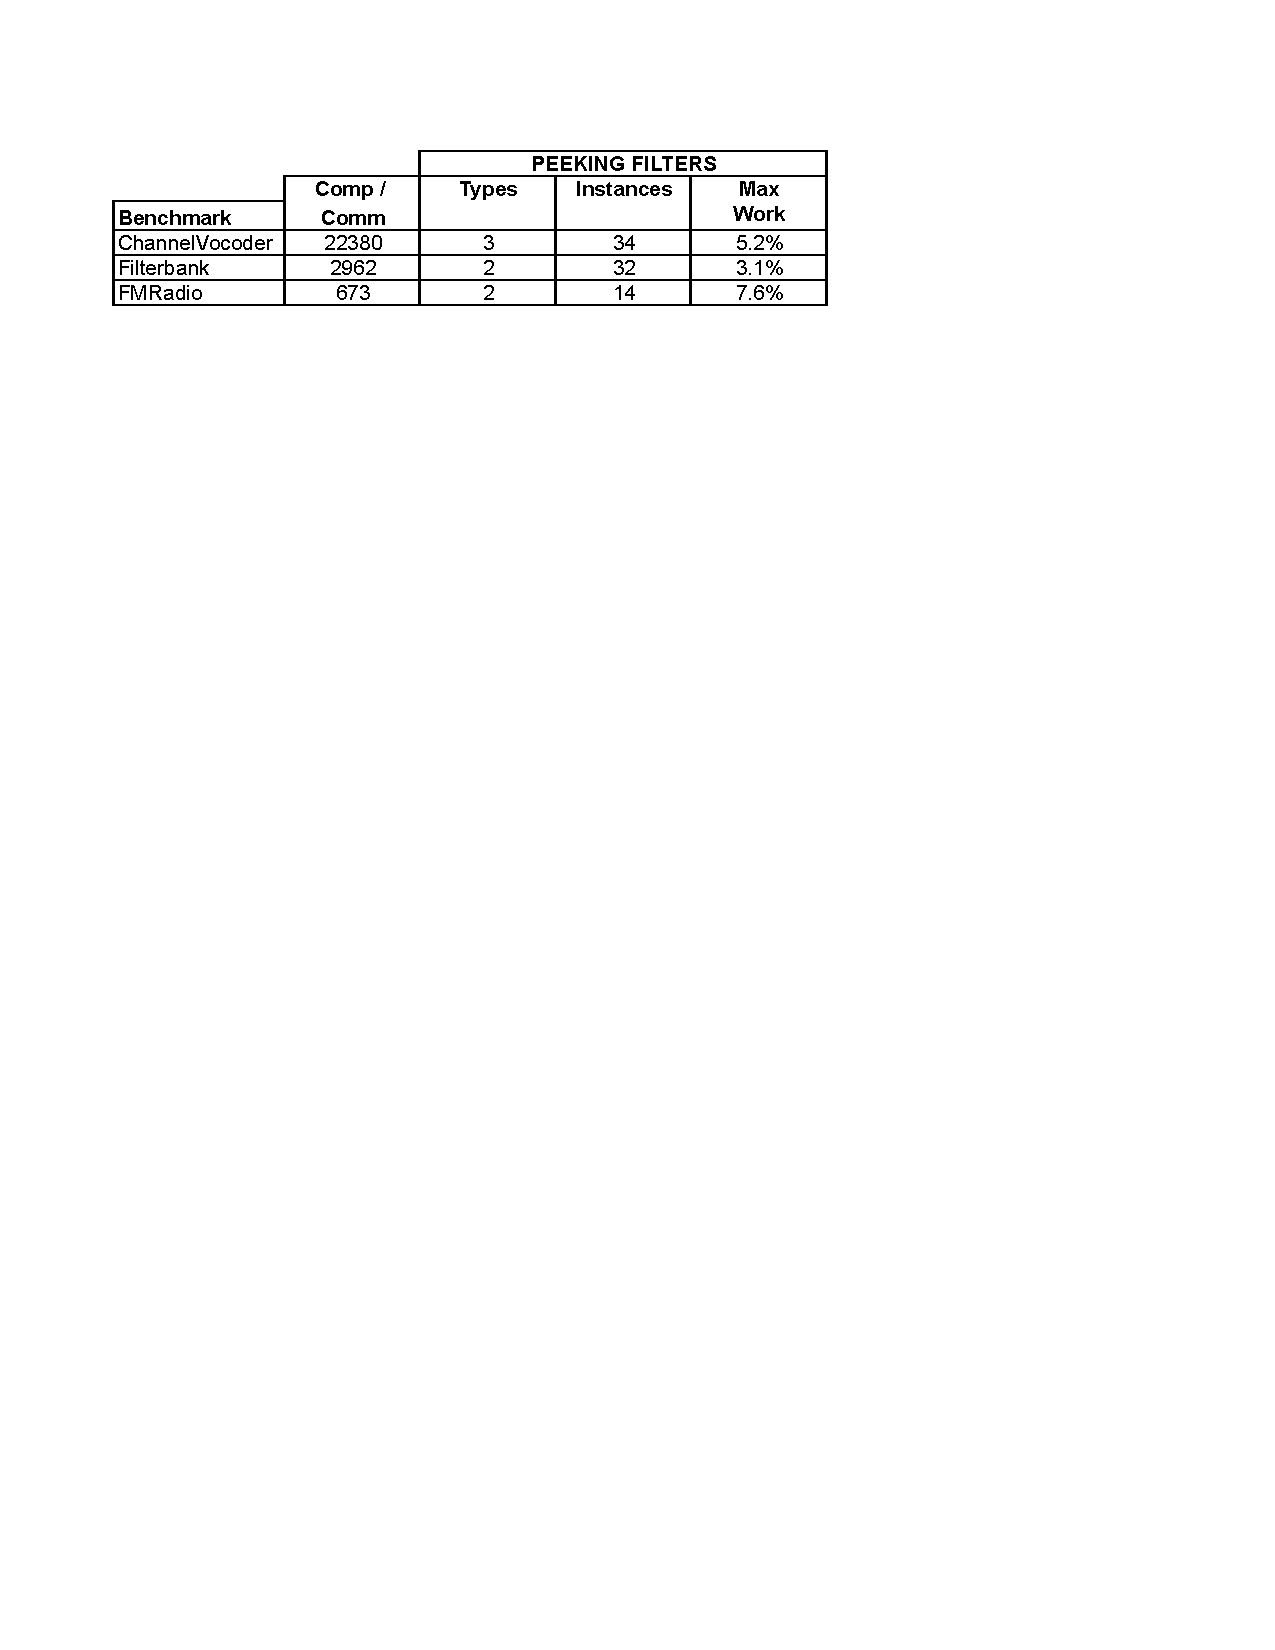
\includegraphics[width=3.3in]{figures/bench-char.pdf}}

\noindent ``Comp/Comm'' provides a static estimation of the
amount of computation to communication ratio by statically estimating the total
work of all the filters and dividing by the number items communicated
for the programmer-conceived graph's steady-state.  The remaining
statistics give the number of peeking filters types, number of peeking
filters instantiated at runtime, and a static estimation of the maximum
work in the single most loaded peeking filter.

We target 2 multicore architecture with different communication
mechanisms.  The Tilera Corporation's TILE64 Processor is a 64 core
system on a chip~\cite{tilera}.  Each core is an identical three-wide
VLIW. The code generated by the StreamIt
compiler for the TILE64 processor follows the remote store programming
(RSP) model~\cite{rsp10} in which each process has a private address
space, but each process can award remote processes write access to
their local memory. When a producer process has write access to a
consumer process's memory, the producer communicates directly with the
consumer via store instructions whose destination is an address in the
consumer's shared memory.  Communication is initiated by the producer,
and is fine-grained.  The consumer reads directly from it's local
memory (L2) when accessing input.

Our symmetric multiprocessor target is a 16-core architecture that is
comprised of four Intel Xeon E7350 multicore processors.  Each processor
is a 64-bit, quad-core with two dual-core dies.  Each die contains a 4
MB L2 cache shared across the two cores.  The front-side bus is clocked
at 1066 MHz.  We utilize the cache coherency mechanism of the
architecture for communication between cores. 

Through empirical experimentation on FMRadio, Filterbank, and
ChannelVocoder, we have settled on $T_{\mt{sharing}} =.10$ and
$T_{\mt{apply}} = 0.05$. These constants are the sweet stop for the two
architectures employed in the experimentation, being a good compromise
between buffer size and inter-core communication.

% \begin{figure*}[t]
% \centering
% \subfigure[]{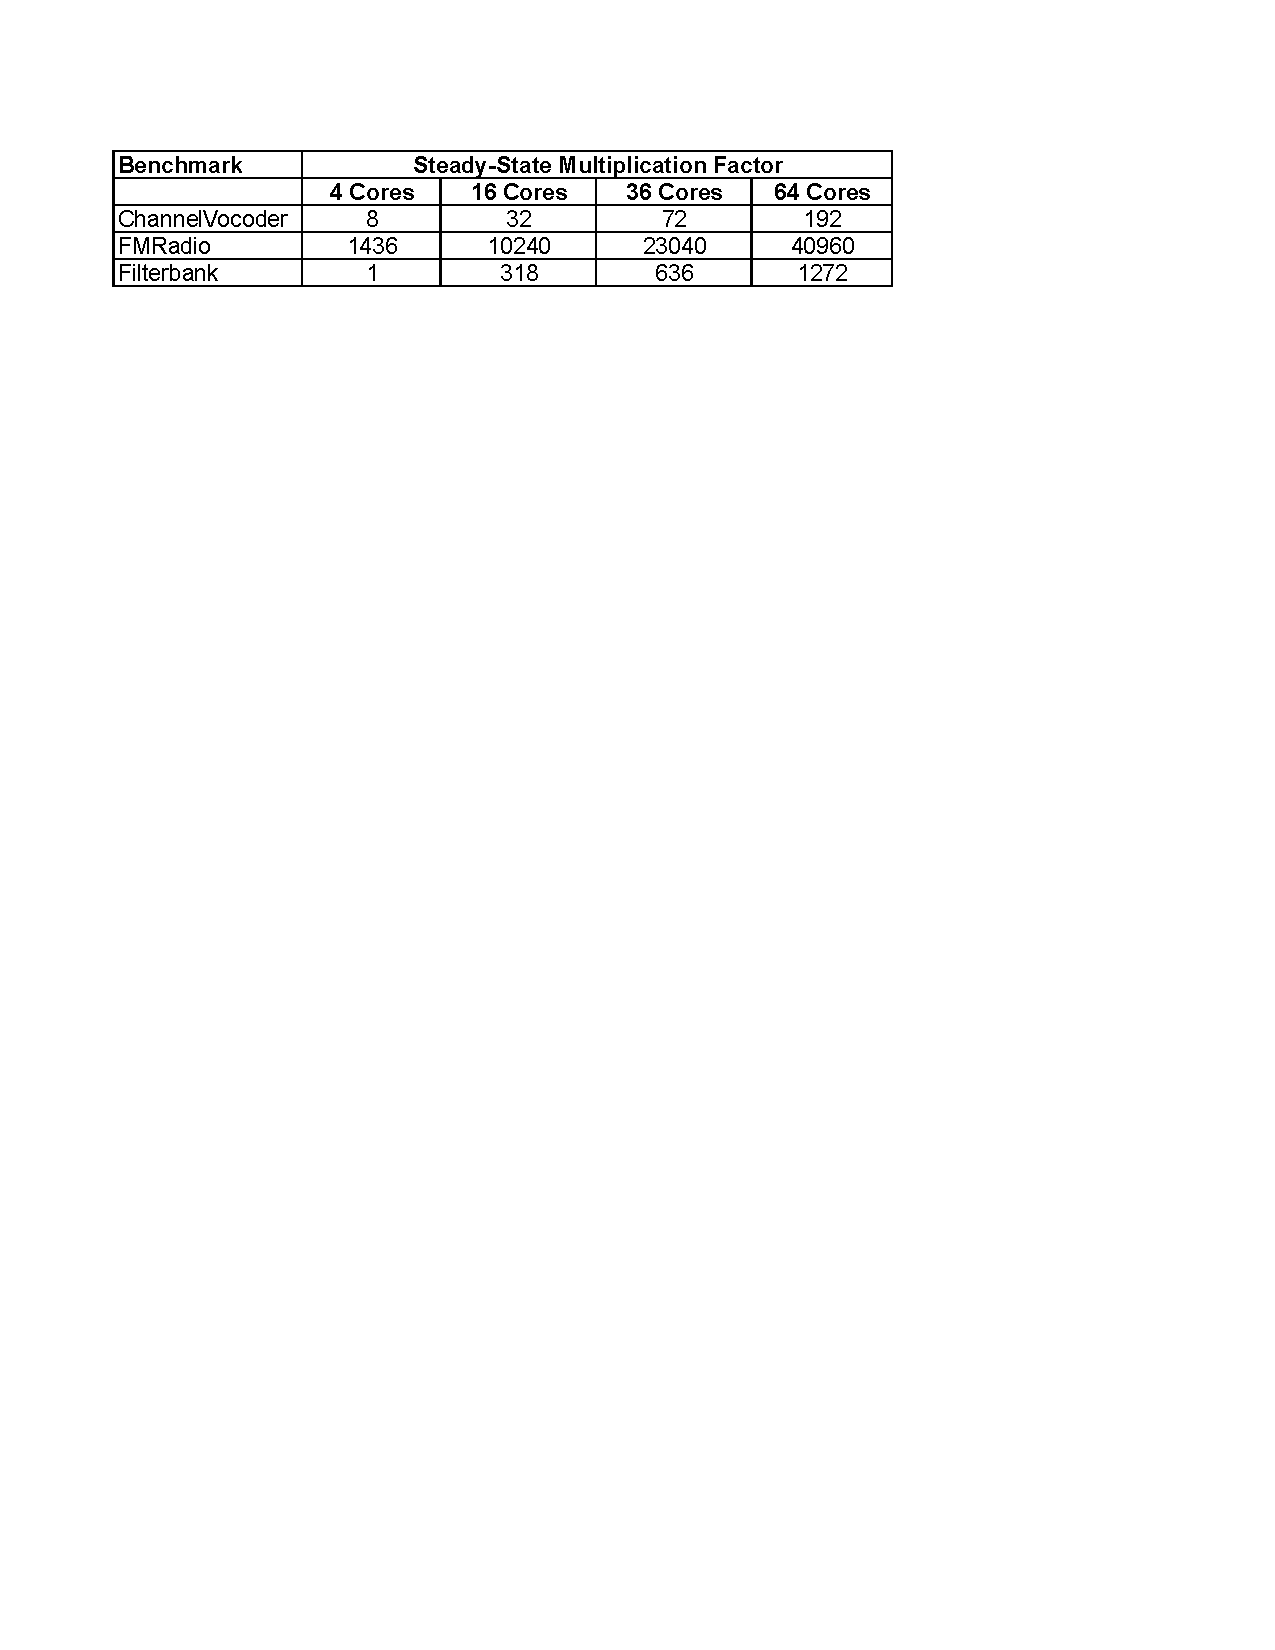
\includegraphics[width=3.7in]{figures/mult-table.pdf}} \\
% \subfigure[]{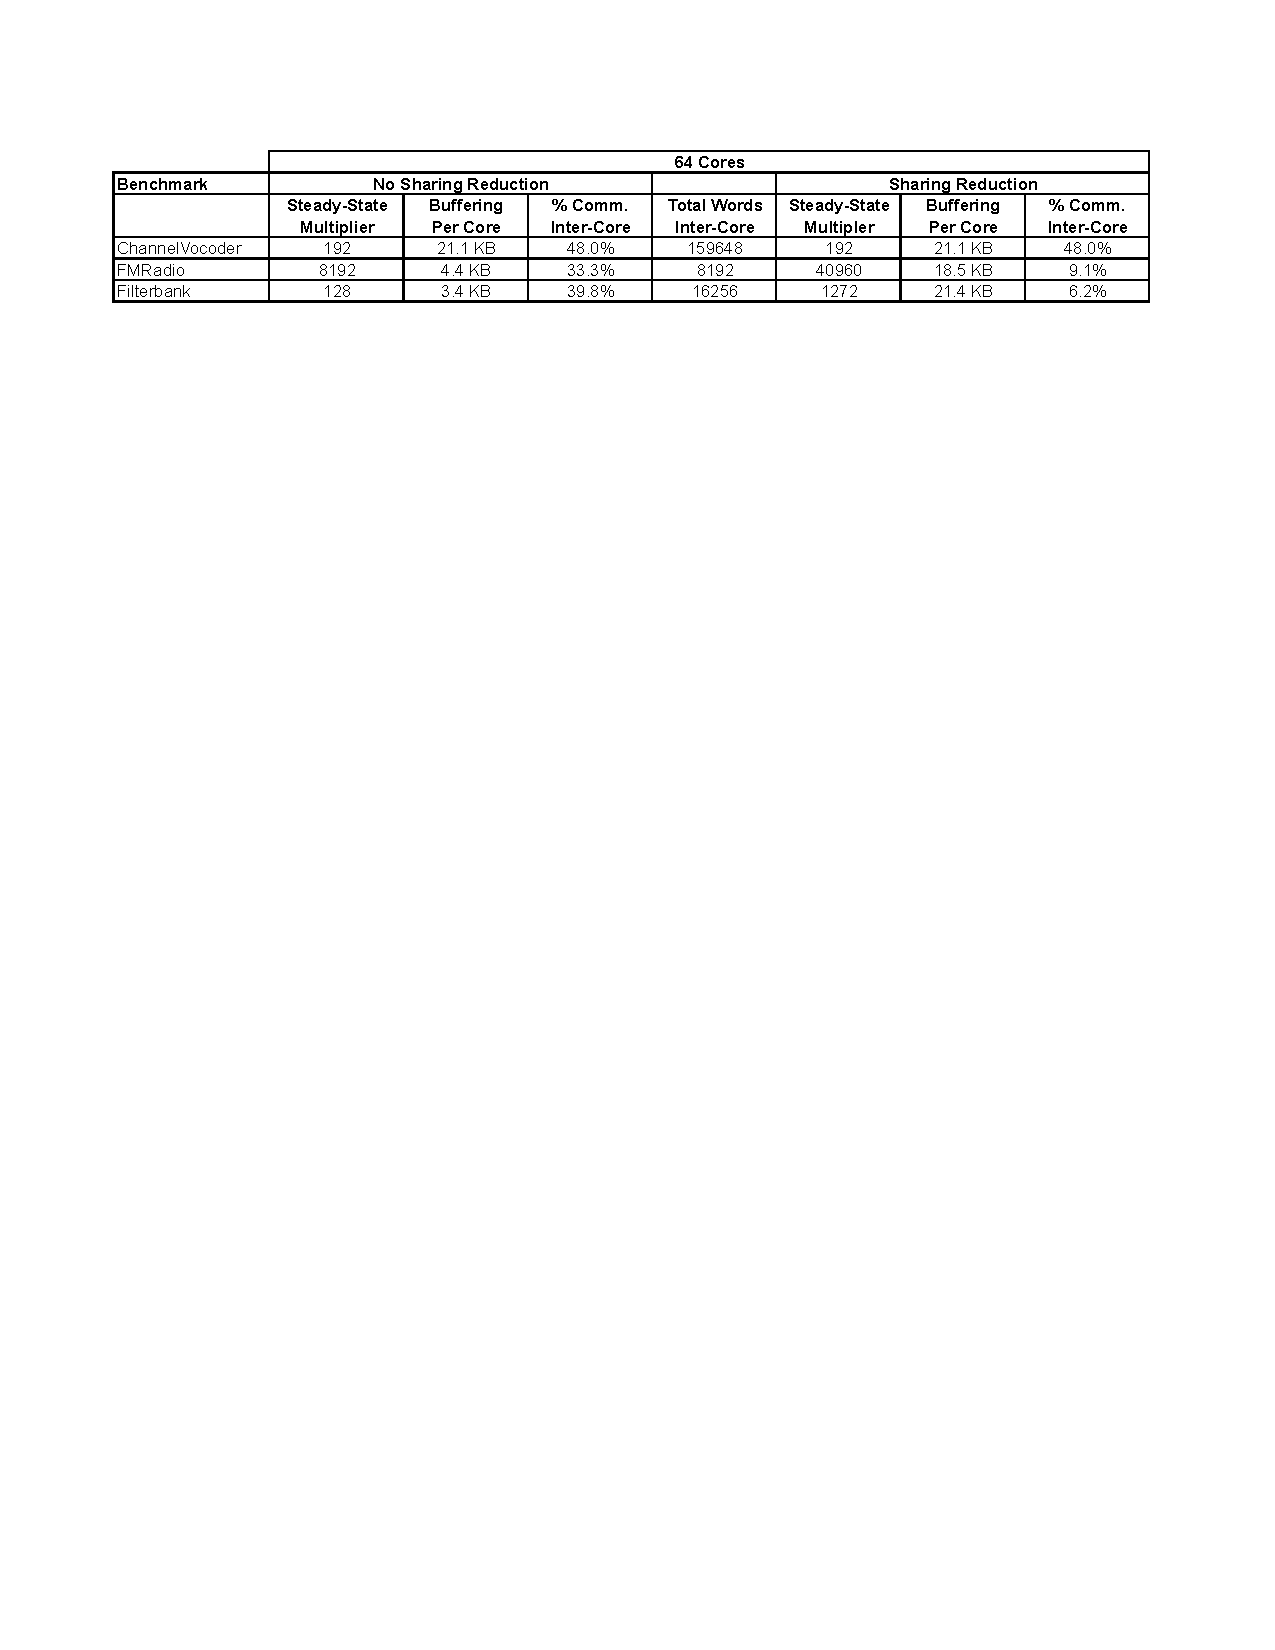
\includegraphics[width=6in]{figures/64-core-table.pdf}}
% \caption[Communication, multiplier and buffering statistics for
% benchmarks.]{
% Communication, multiplier and buffering characteristics for
% benchmarks: (a) gives the steady-state multipliers calculated for
% sharing reduction, (b) compares the steady-state with and without
% sharing reduction. 
% \label{fig:fission-table}}
% \end{figure*}

\begin{figure*}[t]
\centering
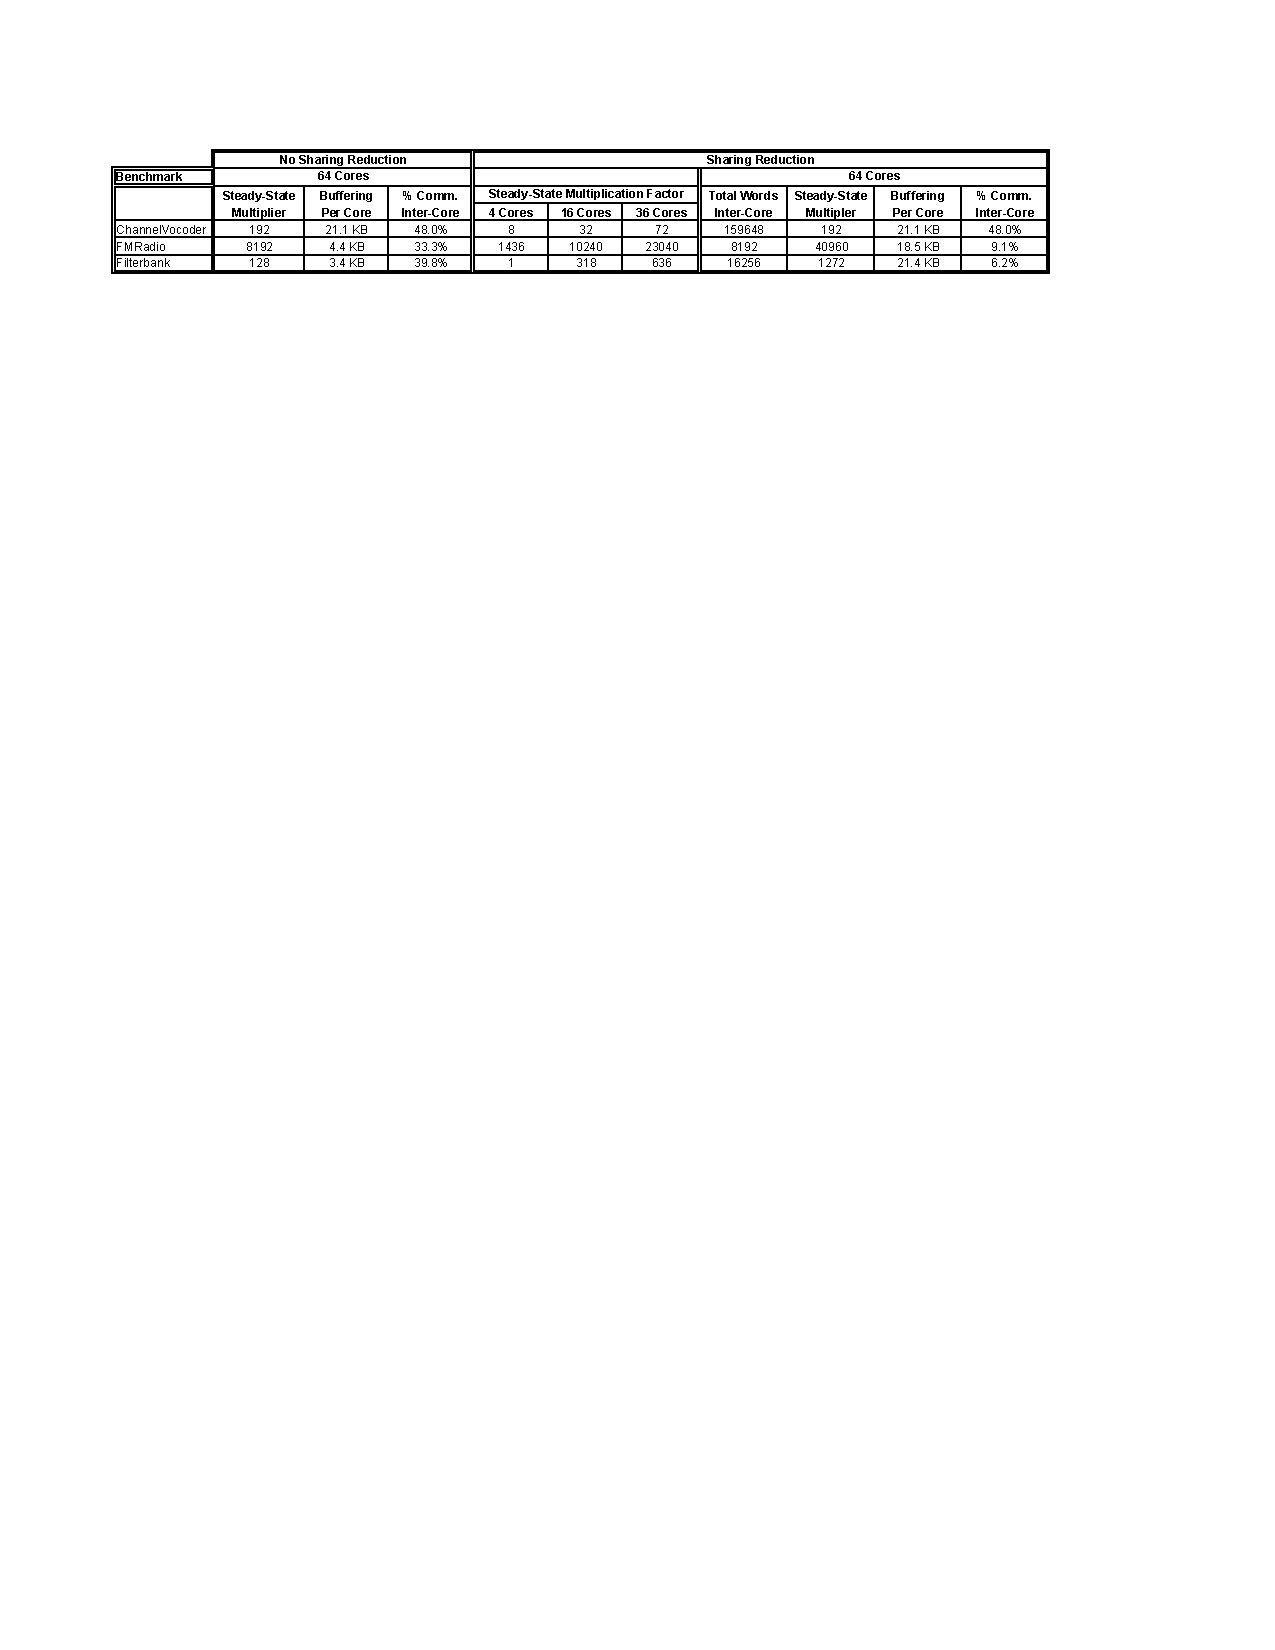
\includegraphics[width=6.1in]{figures/big-table.pdf}
\caption{\label{fig:big-table}  Steady-state multiplicity, buffering,
  and communication for fission with and without sharing reduction.}
\end{figure*}

% \begin{figure}[t]
% \centering
% 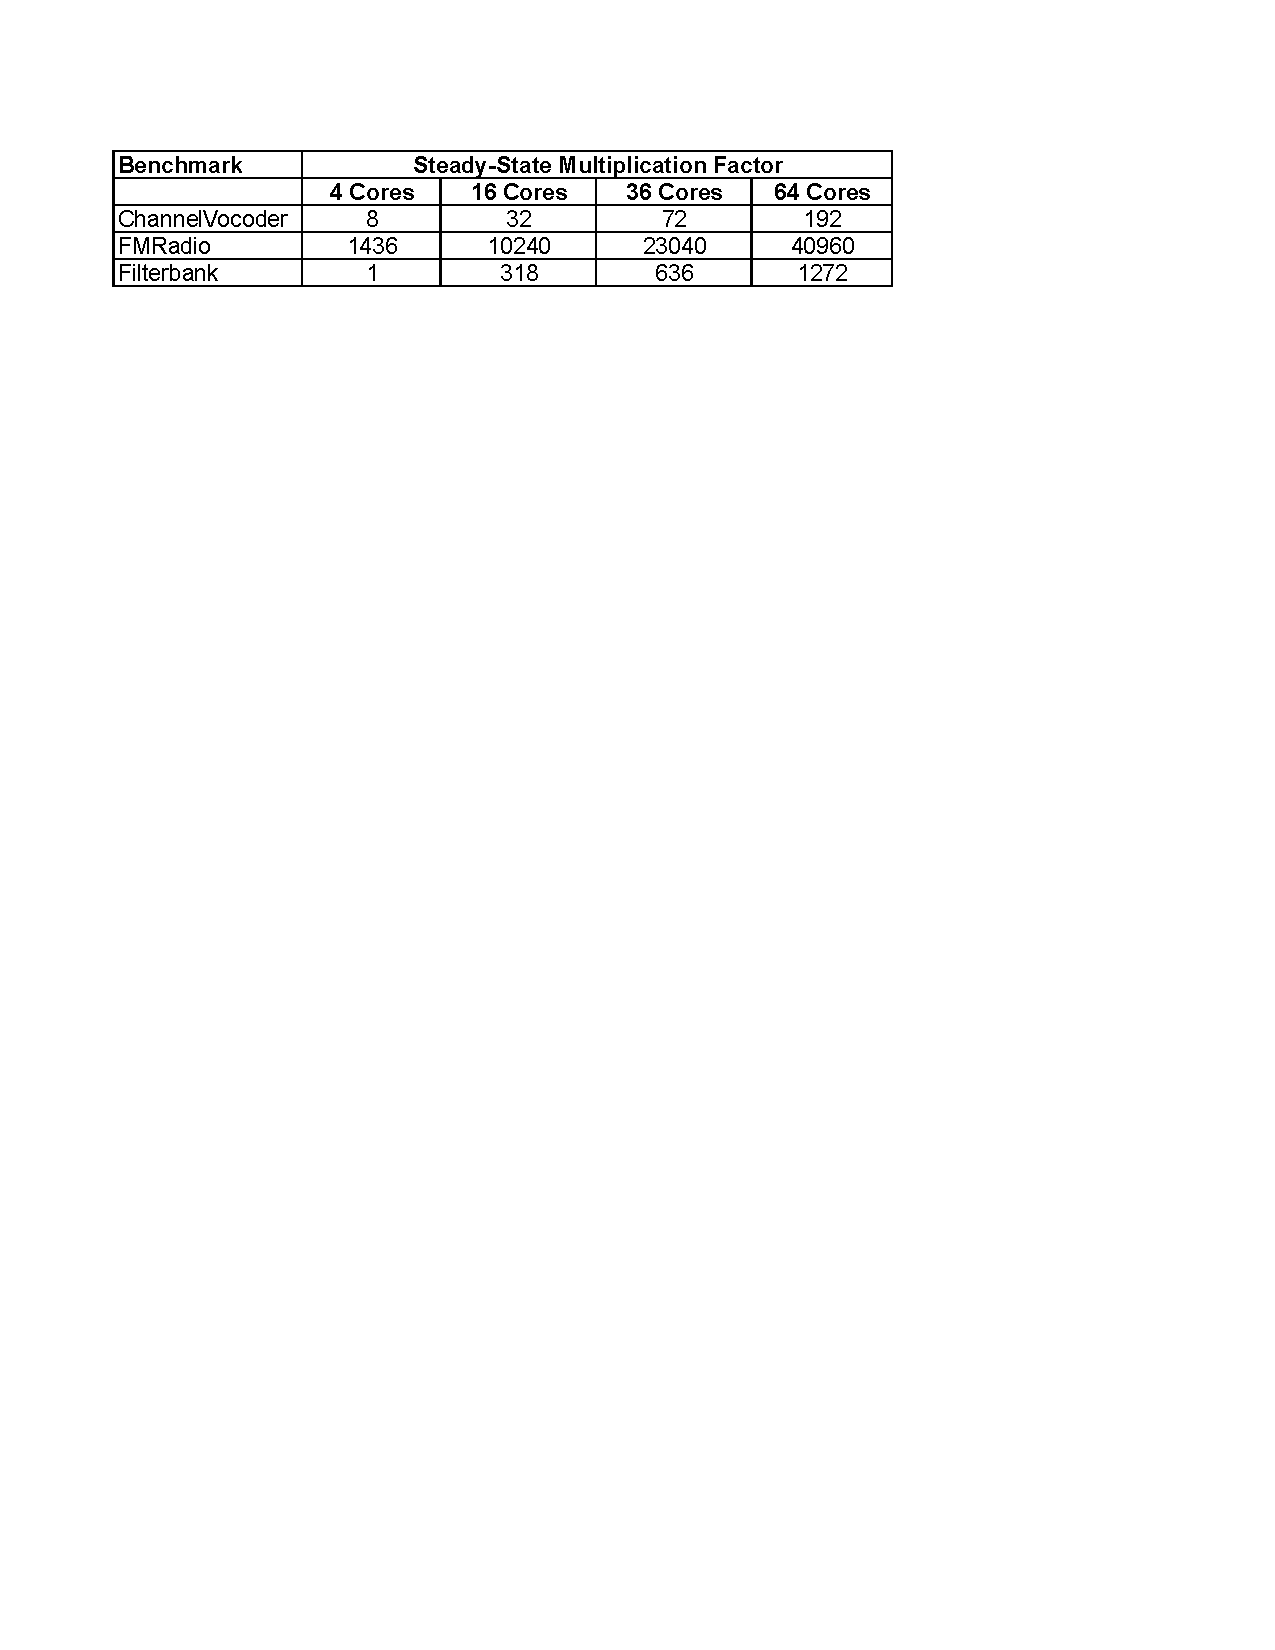
\includegraphics[width=3.3in]{figures/mult-table.pdf}
% \caption{\label{fig:mult-table}  The steady-state multipliers calculated for
% sharing reduction.}
% \end{figure}

% \begin{figure*}[t]
% \centering
% 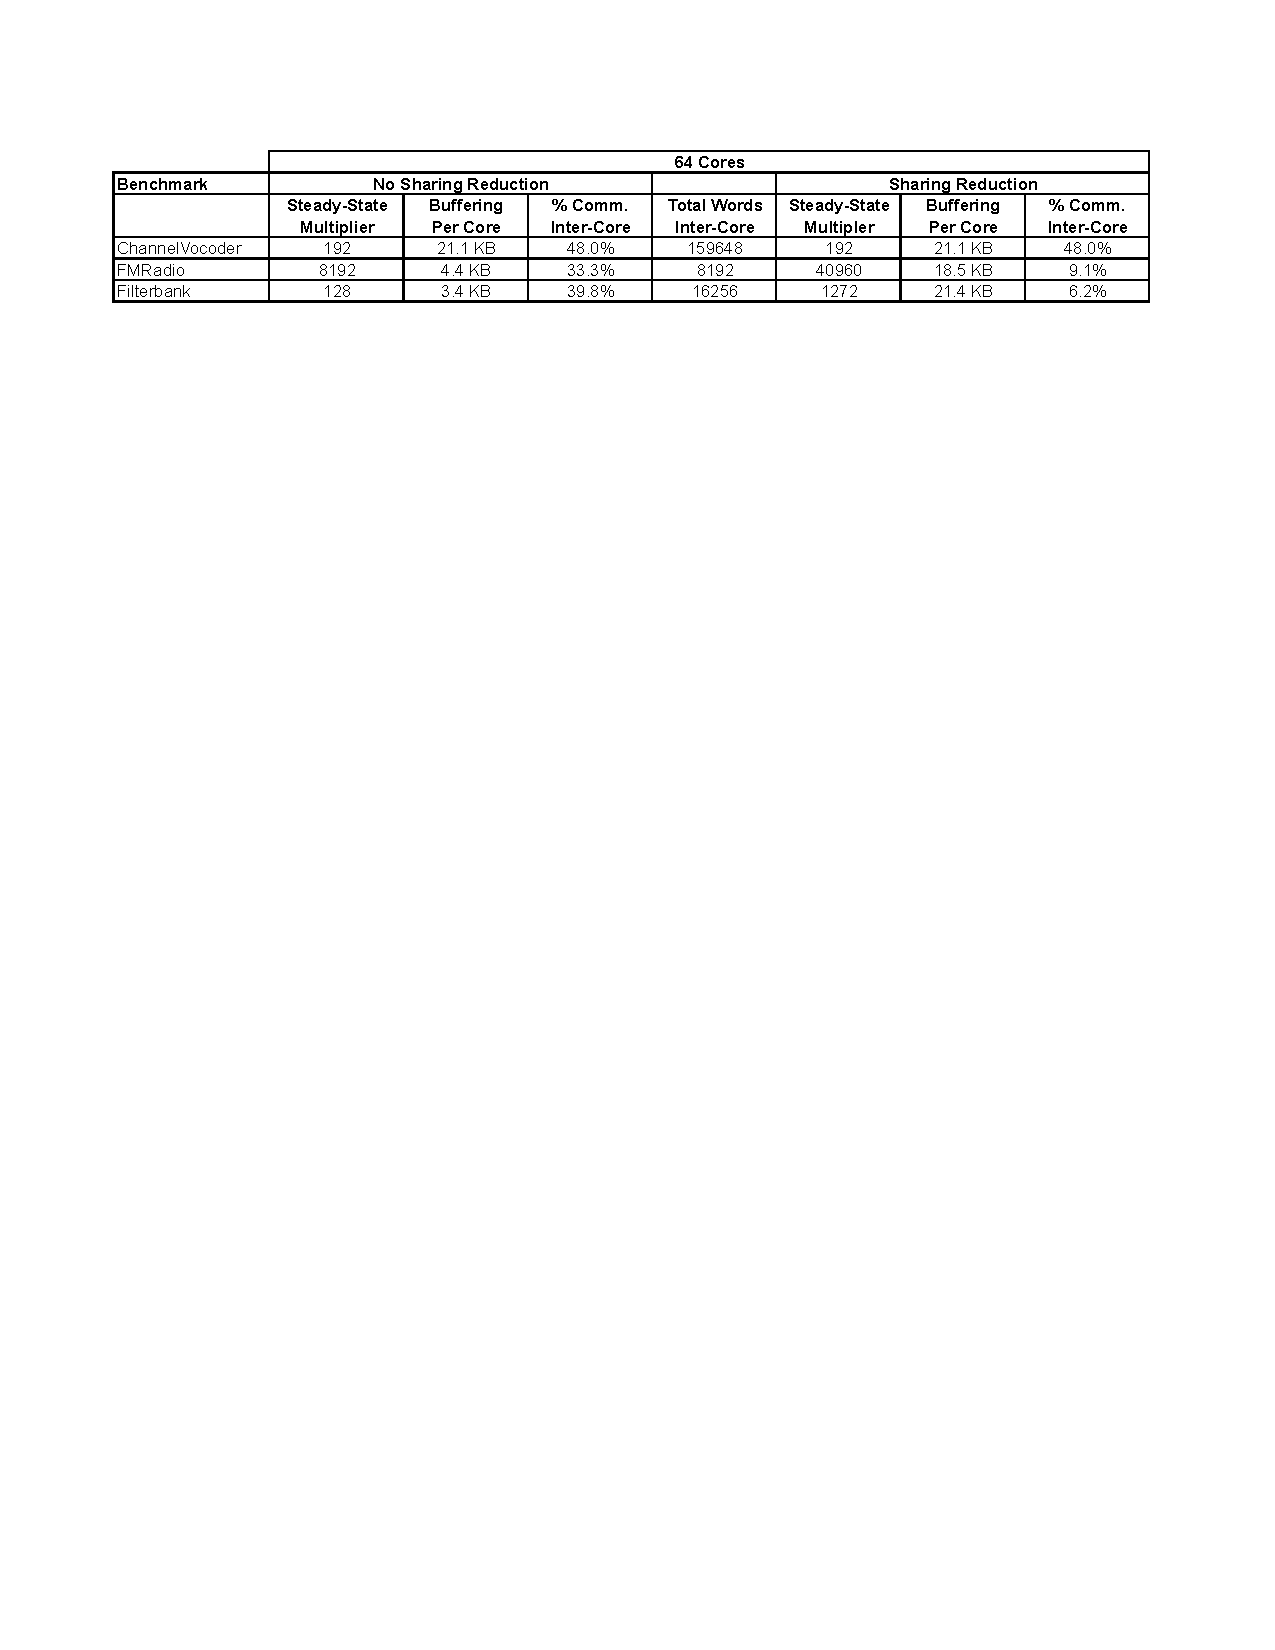
\includegraphics[width=6in]{figures/64-core-table.pdf}
% \caption{ Multiplier, buffering and communication for the steady-state with and without
% sharing reduction. 
% \label{fig:fission-table}}
% \end{figure*}

Figure~\ref{fig:big-table} compares the steady-state with and
without sharing reduction for a 64-core mapping, as well as gives the
constant $c$ calculated by sharing reduction for 4, 16, and 36.  The
factor is larger for FMRadio because one filter has $C(f) \gg o(S,
f)$.  The multiplication factor affects both latency and buffer sizes
adversely.  The application designer will have to decide if the
latency of these techniques can be borne given the application
criteria.  The total buffering requirement is increased when the
steady-state is increased.  However, since we are then fissing, the
buffer is divided amongst the fission products, and the {\it per-core}
buffering requirement is unaffected by the increase.  For example,
FMRadio, has a per-core 18 KB buffering requirement across all
configurations (4, 16, 36, and 64 cores).  This requirement fits in
the per-core L2 size of 64 KB for the Tile64.

 For ChannelVocoder,
sharing reduction has no effect because most of the peeking filters do
not satisfy $T_{\mt{apply}} = 0.05$ because of differing fission
factors between producers and consumers.  For the peeking filters that do,
the steady-state multiplier required for legal general fission for the
graph is enough to assure $T_{\mt{sharing}}$ is met.  Even though
sharing reduction has no effect for ChannelVocoder, general fission
avoids the 38\% of total items that were unnecessary duplicated by
DupDec.

For FMRadio and Filterbank, sharing reduction leads to significant
decreases in the percentage of total items communicated inter-core for
each steady-state.  The buffer requirement is increased an average of
5.2x for these benchmarks.  The total number of words communicated
inter-core during each steady-state is the same, with and without
sharing reduction.  However, the steady-state is greater in the
sharing reduction case, thus producing more outputs.

\begin{figure}[t]
\centering
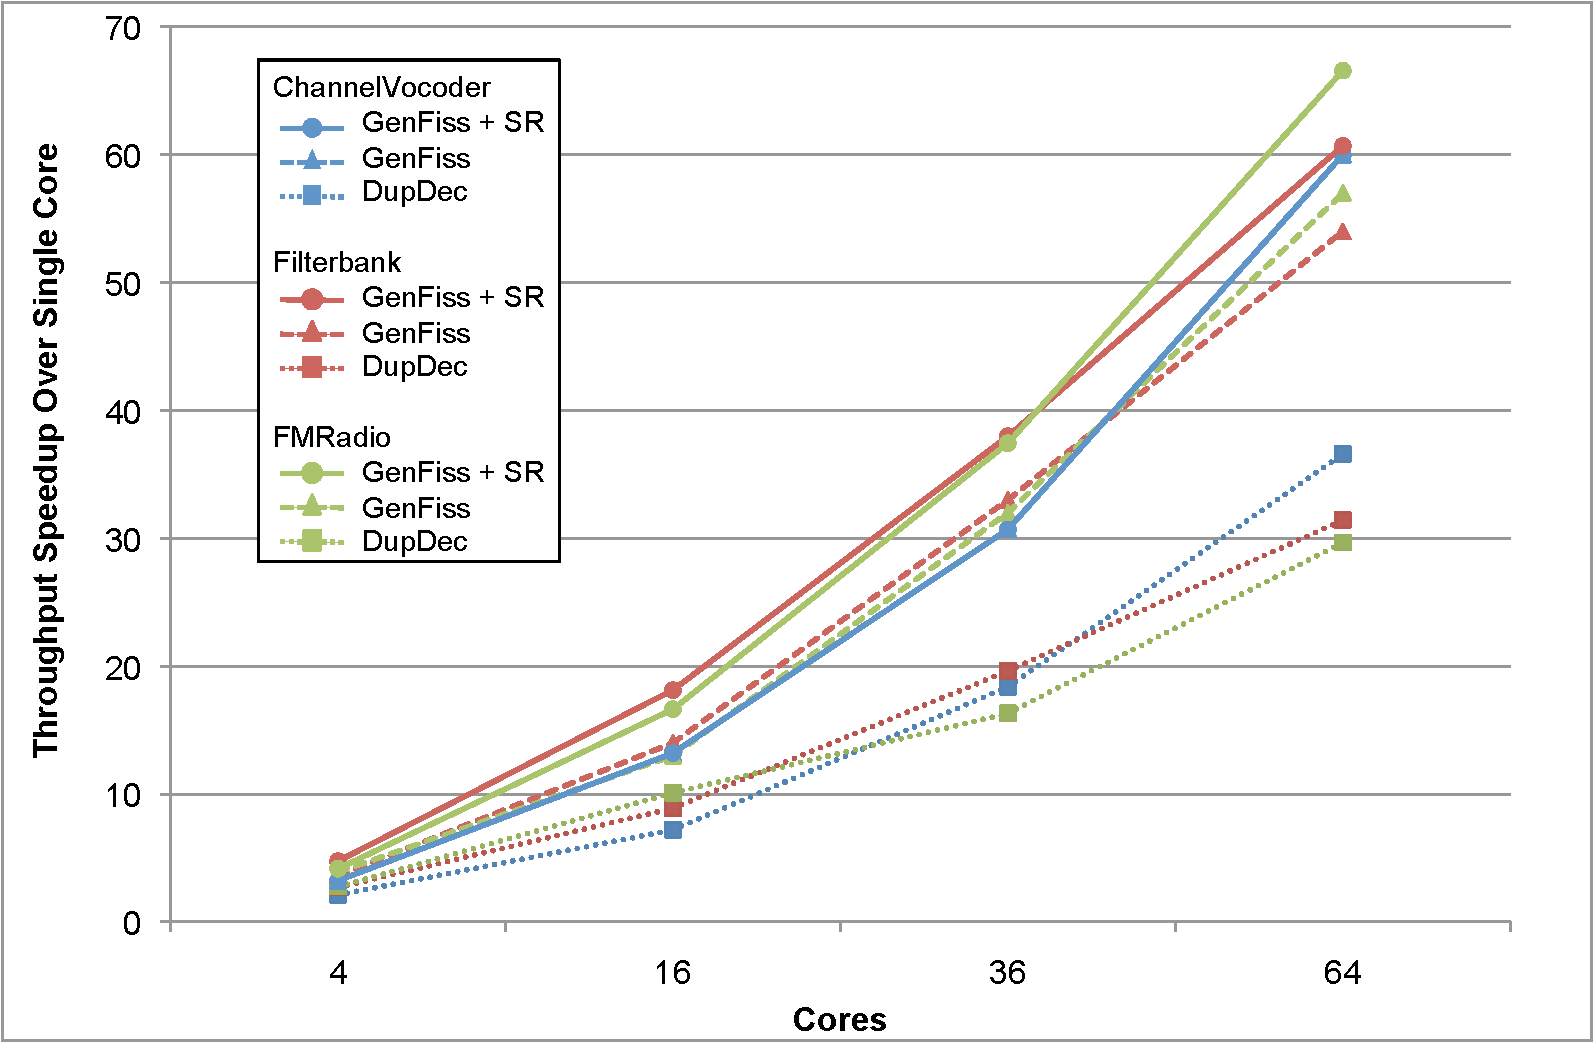
\includegraphics[width=3.3in]{figures/tilera-chart.pdf}
\caption[Comparing the fission techniques on the TILE64.]{
  Evaluation for DupDec versus general fission versus general fission with sharing reduction
  4, 16, 36, and 64 cores on the TILE64.  \label{fig:tilera-chart}}
\end{figure}

Figure~\ref{fig:tilera-chart} gives the performance results for the
Tilera TILE64 architecture.  We present results for DupDec, general
fission, and general fission with sharing reduction for 4, 16, 36, and
64 core configurations, with throughput normalized to single-core
throughput.  General fission with sharing reduction outperforms
DupDec by an average of 1.8x for the three benchmarks when targeting
64 cores. The average 64-core speedup over single core is 62.3x for the
general fission plus sharing reduction for these three benchmarks.

FMRadio experiences the most significant gain from general fission
plus sharing reduction over DupDec (67x versus 30x, respectively, for
64 cores).  FMRadio has the lowest computation to communication ratio
of the 3 benchmarks.  Furthermore, each filter of is fissed by the
number of cores targeted.  For 64 cores, each filter is fissed 64
ways.  DupDec must perform a global all-to-all communication involving
all 64 cores between each level of the graph!
 
ChannelVocoder achieves a 60x speedup for general fission over a
single core.  This is not perfectly linear because of the parallel
mapping; asymmetries exist between the extent of task parallelism and
the number of cores (see~\ref{mgordon-asplos06}).  The speedup over
DupDec (1.62x) is more modest because the width of many of the
fission applications is 3, so DupDec is duplicating input data to
groups of 3 filters.  Filterbank is similar, the width of fission is 4
for all filters when targeting 64 cores.

Sharing reduction is required to achieve scalable speedups for both
FMRadio and Filterbank.  For FMRadio, sharing reductions leads to a
17\% speedup increase for 64 cores.  This because sharing reduction
significantly reduces the number of remote write store instructions
required per output.  This affects FMRadio because of its low
computation to communication ratio.  Sharing reduction sees a 12\%
increase on Filterbank, as Filterbank has a larger computation to
communication ratio.

\begin{figure}[t]
\centering
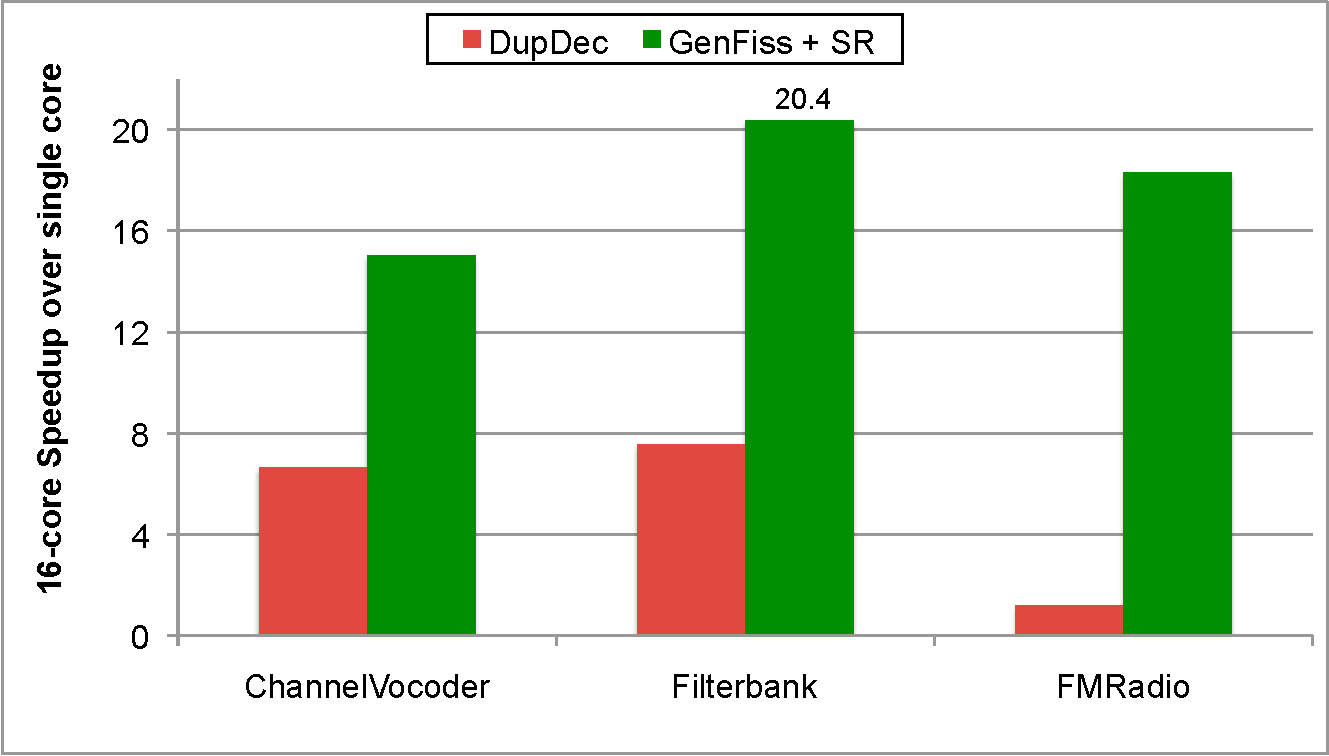
\includegraphics[width=3.3in]{figures/smp-chart.pdf}
\caption[Comparing the fission techniques on the 16-core SMP.]{
  Evaluation for DupDec versus general fission with sharing reduction
  for the 16-core SMP architecture.  \label{fig:smp-chart}}
\end{figure}

Our techniques enable scalable parallelization, with a mean speedup of
17x for our 3 benchmarks on the SMP.  Figure~\ref{fig:smp-chart} gives
the 16-core speedup comparison for DupDec versus general fission with
sharing reduction for our target SMP architecture.  The mean speedup
increase for general fission with sharing reduction over DupDec is
6.7x.  FMRadio again sees the largest speedup increase in the
comparison at 13.0x.  The reasons for this large speedup are similar
as given in the previous section.  However, the SMP communication
mechanism is not as efficient as the TILE64, thus general fission with
sharing reduction gives a greater speedup because reducing inter-core
communication has more impact.

\section{Related Work}
\label{sec:related}

% BILL

%Signal~\cite{Signal}, 
%Lucid~\cite{Lucid77}, and
%Occam~\cite{Occam}, and Sisal \cite{sisal}.
%Parallel Haskell~\cite{ph}
In addition to StreamIt, there are a number of stream-oriented
languages drawing from domains such as functional, dataflow, CSP and
synchronous programming~\cite{survey97}.  The Brook language is
architecture-independent and focusses on data
parallelism~\cite{brook04}.  Stream kernels are required to be
stateless, though there is special support for reducing streams to a
single value.  Stream\-C/Ker\-nel\-C is lower level than Brook;
kernels written in KernelC are stiched together in StreamC and mapped
to the data-parallel Imagine processor~\cite{imagine03ieee}.  SPUR
adopts a similar decomposition between ``microcode'' stream kernels
and skeleton programs to expose data parallelism~\cite{spur05samos}.
Cg exploits pipeline parallelism and data parallelism, though the
programmer must write algorithms to exactly match the two pipeline
stages of a graphics processor~\cite{cg03}.  Compared to these
languages, StreamIt places more emphasis on exposing task and pipeline
parallelism (all the languages expose data parallelim).
%and on sliding window operations (filters that peek).  
By adopting the synchronous dataflow model of execution~\cite{lee87},
StreamIt focusses on well-structured programs that can be aggressively
optimized.  The implicit infinite loop around programs is also a key
StreamIt characteristic that enables the transformations in this
paper.  Spidle is also a recent stream language that was influenced by
StreamIt~\cite{spidle03}.
%and Lucid Synchrone~\cite{Lucid-Synchrone}.
%Synchronous languages which
%target embedded applications include Esterel~\cite{Esterel},
%Lustre~\cite{Lustre}, and Additional

Liao et al. map Brook to multicore processors by leveraging the affine
partitioning model~\cite{liao06brook}.  While affine partitioning is a
powerful model for parameterized loop-based programs, in StreamIt we
simplify the problem by fully resolving the program structure at
compile time.  This allows us to schedule a single steady state using
flexible, non-affine techniques (e.g., simulated annealing) and to
repeat the found schedule for an indefinite period at runtime.
Gummaraju and Rosenblum map stream programs to a general-purpose
hyperthreaded processor~\cite{gummaraju05micro}.  Such techniques
could be integrated with our spatial partitioning to optimize per-core
performance.  Gu et al. expose data and pipeline parallelism in a
Java-like language and use a compiler analysis to efficiently extract
coarse-grained filter boundaries~\cite{du03sc}.  Ottoni et al. also
extract decoupled threads from sequential code, using hardware-based
software pipelining to distribute the resulting threads across
cores~\cite{ottoni05decoupled}.  By embedding pipeline-parallel
filters in the programming model, we focus on the mapping step.

%%%%%%%%%%%%%%%%%%%%%%%%%%%%%%%%%%%%%%%%%%%%%%%%%%%%%%%%%%%%%%%%%%%%%

Previous work in scheduling computation graphs to parallel targets has
focused on partitioning and scheduling techniques that exploit task
and pipeline parallelism~\cite{SDFSched, SDFSched2,may87communicating,
DAGSched, pipeline-sdf}.  Application of loop-conscious
transformations to coarse-grained dataflow graphs has been
investigated.  Unrolling (or ``unfolding'' in this domain) is employed
for synchronous dataflow (SDF) graphs to reduce the initiation
interval but they do not evaluate mappings to actual
architectures~\cite{unfolding,unfolding2}. Software pipelining
techniques have been applied to SDF graphs onto various embedded and
DSP targets~\cite{bakshi99,chatha-02}, but has required programmer
knowledge of both the application and the architecture. To our
knowledge, none of these systems automatically exploit the combination
of task, data, and pipeline parallelism.  Furthermore, these systems
do not provide a robust end-to-end path for application
parallelization from a high-level, portable programming language.

%% Previous work on instruction-level software pipelining has focused
%% mostly on scheduling machine instructions in a loop via modulo
%% scheduling~\cite{rau81,lam-softpipe}.  The algorithms devised must
%% account for tight resource constraints and complex instruction
%% dependences. Our software-pipelining problem is much less constrained,
%% enabling us to employ a simple greedy heuristic.  

%% Furthermore, a traditional modulo scheduling algorithm is not needed
%% because we have an implicit loop barrier at the end of each
%% steady-state.  ILP compilers for clustered VLIW
%% architectures~\cite{Bulldog,Multiflow,lee98spacetime,qian02} must
%% partition instructions and assign them to clusters as part of the
%% instruction scheduling. Clustering is analogous to our application of
%% filter fusion in our software pipelining algorithm.

\section{Conclusion}
\label{sec:conclusion}

In this paper, we describe the StreamIt compiler for the Raw
architecture.  The stream graph of a StreamIt program exposes the data
communication pattern to the compiler while the lack of global
synchronization frees the compiler to radically reoganize the program
for efficient execution on the underline architecture. The StreamIt
compiler demonstrates the power of this flexibility by totally
reoganizing large programs for better load balance. We were able to
map many of programs on to the Raw processor and obtain good
performance.

We introduce a collection of optimizations, vertical and horizontal
filter fusion, vertical and horizontal filter fission and filter
reordering transformations, that can be used to restructure stream
graphs.  We show that by applying these transformations we can map a
high-level stream program, written to reflect the composition of the
application, onto Raw and achieve good processor utilization and load
balance, leading to a factor of three speedup on two applications.

Unlike all previous streaming languages, the structured streams of
StreamIt makes it possible for us to approach the optimization and
parallelization problems in a very systermatic manner. It enables us
to define multiple optimizations -- targetting different constructs
and requirements -- and to compose them them in a hirearchical manner.

The ability to do global transformations across multiple filters, that
may have originated from very different parts of the application,
makes it possible for the compiler to find optimization opportunities
that may ellude even an experience programmer.  Such capabilities
enables the programmers to write protable streaming applications and
map them efficiently onto any given architecture. This has the
potential of creating a programming standard for emerging
communication exposed architectures.  The StreamIt compiler takes a
fist step towards this goal.



% \acks
% Acknowledgments, if needed.

% We recommend abbrvnat bibliography style.
\footnotesize
\bibliography{references}
\bibliographystyle{abbrvnat}

% The bibliography should be embedded for final submission.

% \begin{thebibliography}{}
% \softraggedright

% \end{thebibliography}

\end{document}
